\chapter{Performance of OOD detectors on~the~simulated data}
\label{chapter:simulations}

This chapter contains the description of the conducted numerical study. The~research was focused on comparing the performance of various algorithms (outlierness measures) for detecting the out-of-distribution data and their ability to properly recognize the~data coming from the same distribution as the training set. The different properties of~these algorithms were observed as an effect of considered parameters changes, such as the~number of training samples, dimension of feature vectors, number of correlated features and the variance value of features. The performance was analyzed in terms of ID-OOD separability, expressed as AUROC score, as well as the classification results (sensitivity, specificity) using threshold calibrated at $95\% TPR$ with respect to the training data. Finally, performed the analysis of errors related to (in)accurate representations of training data by the outlier detectors, considering the influence of the feature space dimensionality and the number of samples. The involved data organization (number of training samples, dimension of feature vectors, Multivariate Normal Distribution) reflects the characteristics of (some) data from the subsequently analyzed real-world benchmark (chapter \ref{chapter:real-data}).

\cleardoublepage{}


\section{Baseline – samples, dimensions and distances}
\label{section:distributions-experiment}

The goal of the first conducted experiment is to observe the behavior of selected outlierness measure and analyze their performance in the outlier detection task –~and to establish the baseline for more specific examinations, performed in further sections. The~effect of~three major parameters is considered: number of training samples $n$, dimension of feature vectors $d$ and the distance to out-of-distribution samples $h$; additionally utilized three different generator distribution functions to produce the data clusters – for even more versatile insight.

It should be noted that the organization of the simulated numerical study includes the ranges of $n$ and $d$ parameters values which are encountered in common OOD detection benchmarks for image and text recognition using Deep Learning models (chapter \ref{chapter:real-data}).


\subsection{Experiment organization}
\label{section:distributions-organization}

The experiment is organized as follows:
\vspace{-0.5\baselineskip}
\begin{itemize}
    \item First, 3 data clusters are generated.
          \begin{itemize}
              \item The set of \underline{training} data $T$, representing the in-distribution (ID) data, containing $n$ samples of dimension $d$, produced from a~chosen generator~$G$ (\textit{Gaussian}/\textit{MVN}, \textit{triangular} or \textit{uniform} distribution – that is located around the~center of~the coordinate system $\mu = [0, 0, \dots, 0]$ with spread of $\pm 1$).
              \item The set of \underline{known} data $K$, representing a testing dataset (another examples of~ID~data), generated from the same distribution as $T$, with a~fixed number of $1000$ samples. It is used to analyze the sensitivity of the detector, i.e., the~ability to properly recognize testing data as similar to the training data.
              \item The set of \underline{unknown} data $U$, representing out-of-distribution (OOD) data and consisting of a~fixed number of $1000$ samples, produced by the same generator as $T$, however with the distribution center shifted by the distance $h$~in~space (so the mean is at location $[\frac{h}{\sqrt{d}}, \frac{h}{\sqrt{d}}, \dots, \frac{h}{\sqrt{d}}]$). It is used to evaluate the specificity of the algorithm (i.e., proper detection of OOD samples).
          \end{itemize}
    \item The selected algorithm $OF$ (Outlier Factor) is fitted to the training dataset $T$.
    \item Next, the outlierness scores are calculated for each element of sets $T$, $K$ and $U$.
    \item The separability between clusters $K$ and $U$, using the selected $OF$, is analyzed by~calculating the Area Under the Receiver Operating Characteristic (AUROC).
    \item The classification of data from clusters $K$ and $U$ with respect to the dataset $T$ and outlierness measure $OF$ is performed, using the threshold value $t$ selected as the 95th and the 99th percentile of outlierness scores obtained for the cluster $T$.
\end{itemize}

Summarizing, the input parameters that vary in the experiment are: number of training samples $n$, dimension of feature space $d$, distance to the outliers $h$, outlierness measure $OF$ and the generator distribution $G$.

Additionally, for each combination of parameters, the experiment was repeated several times with various values of the generator seed $\xi$ (that affected the values within $T$, $K$ and $U$) to observe the variability of results.


\subsection{Experiment results – distribution properties}
\label{section:distributions-results-properties}

The aim of the first experiment was to analyze the behavior and usability of selected outlierness measures, discussed in section \ref{section:measures}, especially when applied in high-dimensional feature spaces, considering such factors as the number of training samples used to model the in-distribution data.

The study shows that various techniques used to model the in-distribution data, such~as~Euclidean distance (ED, section \ref{section:Euclidean}), Integrated Rank Weighted Depth (IRWD, section \ref{section:IRWD}), k-Nearest Neighbors (kNN, section \ref{section:kNN}) and Local Outlier Factor (LOF, section \ref{section:LOF}), have completely different properties. Although all of them can be considered as distance metrics, their output values are not directly comparable, e.g., the same element $v$ can obtain score $s=20$ using Mahalanobis distance (MD, section \ref{section:Mahalanobis}) and score $s=-0.65$ with Angle-Based Outlier Factor (ABOF, section \ref{section:ABOF}). Hence, selecting any arbitrary threshold value $t$ for distinguishing outliers, without additional analysis, is not universally possible.

Figure \ref{fig:histograms} presents example distributions of scores obtained for six different outlierness measures: ABOF, ED, IRWD, kNN, MD and LOF. First major difference between the techniques that can be noticed is in the ranges of values – as ED, kNN and MD are directly related to the spatial distances, the values are greater than for ABOF, IRWD and LOF, that rely on other quantities (variances scaled by distances, depth estimations with projections and comparison of neighbors' local reachability densities). The~results obtained for Standardized Euclidean distance (SED, section \ref{section:SEuclidean}) are nearly the same as for ED, due to the variance set to $1.0$ in the experiment, hence they are omitted and not presented in~figure~\ref{fig:histograms}.

It is worth to notice that from all considered measures only the IRWD is characterized by a limited range of the function value domain. For all other measures, there is either no upper limit or no lower limit.
\vspace{-0.5\baselineskip}
\begin{itemize}
    \item ABOF: $s \in \left(-\infty, 0.0\right]$,
    \item IRWD: $s \in \left[-0.5, 0.0\right]$,
    \item ED, kNN, LOF, MD, SED: $s \in \left[0.0, +\infty\right)$.
\end{itemize}
\vspace{-0.5\baselineskip}
Note that the score values of ABOF and IRWD are negative in this study, because in~implementation (Appendix \ref{chapter:source-code}) the returned values of formulas \ref{eq:abof} and \ref{eq:irwd} are inverted (multiplied by $-1$) to satisfy the criteria given by formula \ref{eq:open-set-classification} (section \ref{section:procedure}) –~i.e.~having greater values to indicate the outliers.

For most of measures (ED, IRWD, kNN, MD) the distributions appear symmetrical. However, in case of LOF the positive skew can be observed (the longer tail is on the right) in case of in-distribution data (train and known data in figure \ref{fig:histogram-lof}). Similarly, for ABOF the distributions are characterized by the negative skew (longer tail on the left side), especially in case of the distant out-of-distribution examples (unknown data in figure \ref{fig:histogram-abof}). This phenomenon is more clearly visible in figure \ref{fig:boxplots}.

The most important observation here is that for some algorithms, notably kNN and MD, the observed outlierness score values for known in-distribution samples (cluster $K$, i.e.~testing data) appear surprisingly distant from the values obtained for the training samples (cluster $T$). This means, that considering only the training samples' perspective (green barplots in figures \ref{fig:histogram-knn} and \ref{fig:histogram-mahalanobis}), most testing data coming from exactly the same distribution (blue barplots in the same figures) would be considered as out-of-distribution, i.e., outliers.

This phenomenon appears algorithm-specific and is observed regardless of generator distribution $G$, i.e., for $\textit{Gaussiann}$ (figures \ref{fig:histogram-knn} and \ref{fig:histogram-mahalanobis}), $\textit{Triangular}$ (figures \ref{fig:hists-knn-triangular} and \ref{fig:hists-md-triangular}) and $\textit{Uniform}$ (figures \ref{fig:hists-md-triangular} and \ref{fig:hists-md-uniform}). For both kNN and MD the effect intensifies in high-dimensional feature spaces (figure \ref{fig:hists-dimensions}). For MD the effect can be suppressed by increasing the number of training samples $n$, as visible in figure \ref{fig:hists-md-samples}, however for kNN the increased $n$ does not impact this phenomenon significantly (figures \ref{fig:hists-knn-500}, \ref{fig:hists-knn-1000} and \ref{fig:hists-knn-5000}). Inn case of kNN, the effect is reduced when greater number of $k$ neighbors is~considered (figure \ref{fig:hists-knn20-1000}).

The same effect can be observed for ED, SED and IRWD measures when the number of training samples $n$ is lower than the dimension of features space $d$, as visible in the figure \ref{fig:hists-extreme-bad} – just like for MD, increasing the number of training samples $n$ causes scores for in-distribution data (clusters $K$ and $T$) to overlap. It is caused by difficulty of obtaining accurate representation of a~cluster in high-dimensional features spaces, discussed further in section \ref{section:overlapping-experiment}. However, surprisingly, this effect was not observed in case of ABOF and LOF measures, even in case of extreme conditions, such as dimension of feature vectors $d = 5000$ and number of training samples $n = 50$, like shown in~the~figures~\ref{fig:hists-extreme-good}.

Despite that the training samples (cluster $T$) may appear distant from the known in-distribution samples (cluster $K$), in all discussed cases there is a~possibility to achieve a~good separation between in-distribution data and outliers (cluster $U$). Hence, the Receiver Operating Characteristic (ROC) curves presented in figure \ref{fig:rocs} look similar –~they present the relation between the sensitivity (True Positive Rate – TPR) and risk of type I error (False Positive Rate).

The ideal separation is reached in case of correct recognition of all in-distribution data without any spurious assignments of outliers – corresponding with top-left corner in ROC plot ($TPR = 1$, $FPR = 0$). The optimal threshold point marked in ROC plot is related to the threshold value that is closest to ideal situation (top-left ROC corner) – represented with the red cut-off vertical lines in figure \ref{fig:histograms}. The second marked threshold, TPR95, corresponds to a cut-off value for which the 95\% of in-distribution data were properly recognized.

The commonly used measure to evaluate the performance of classification model is the calculated Area Under the Receiver Operating Characteristic (AUROC) curve, with ideal value being $AUROC = 1.0$; any value $AUROC \leq 0.5$ means the classifier is worse than randomly performed assignments. In figure \ref{fig:rocs} all AUROCs are greater than $0.9$, indicating very well separation between clusters $K$ and $U$.

\begin{figure}[t]
    % StreamLit settings: width=5, height=3
    \centering
    \begin{subfigure}[b]{0.495\textwidth}
        \centering
        \caption{\small Angle-Based Outlier Factor}
        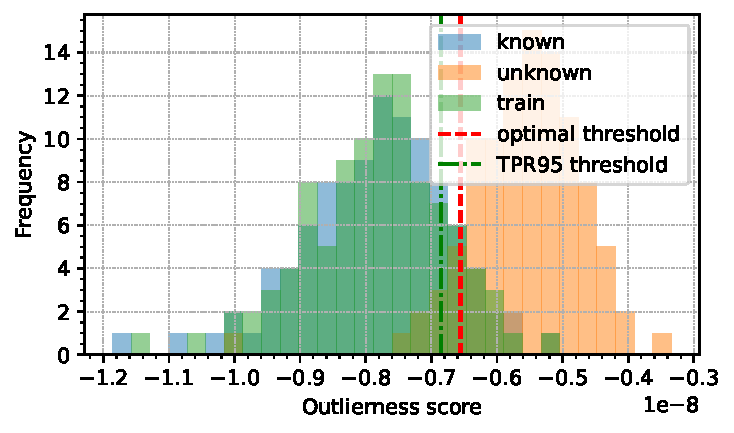
\includegraphics[width=\textwidth]{images/distributions/histograms/hist-distributions-dimension_250-samples_1000-distance_8-distribution_gaussian-model_ABOF-seed_0.pdf}
        \label{fig:histogram-abof}
    \end{subfigure}
    \hfill
    \begin{subfigure}[b]{0.495\textwidth}
        \centering
        \caption{\small Euclidean distance}
        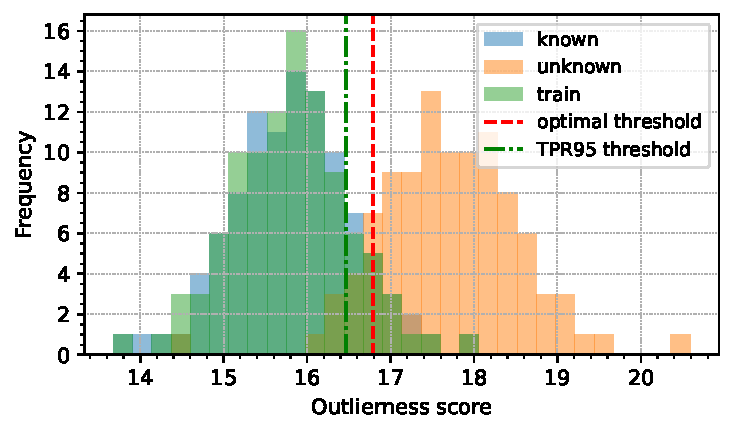
\includegraphics[width=\textwidth]{images/distributions/histograms/hist-distributions-dimension_250-samples_1000-distance_8-distribution_gaussian-model_ED-seed_0.pdf}
        \label{fig:histogram-euclidean}
    \end{subfigure}
    \begin{subfigure}[b]{0.495\textwidth}
        \centering
        \caption{\footnotesize Integrated Rank Weighted Depth ({\scriptsize$n_{proj} = 10^3$})}
        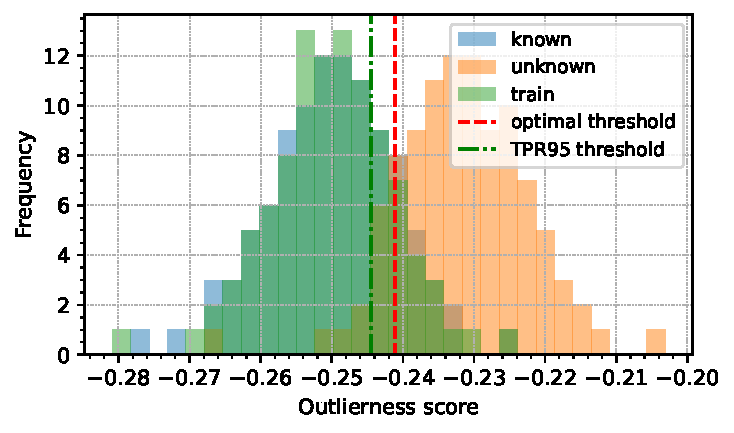
\includegraphics[width=\textwidth]{images/distributions/histograms/hist-distributions-dimension_250-samples_1000-distance_8-distribution_gaussian-model_IRWD-1000-seed_0.pdf}
        \label{fig:histogram-irwd}
    \end{subfigure}
    \hfill
    \begin{subfigure}[b]{0.495\textwidth}
        \centering
        \caption{\small k-Nearest Neighbors ($k=10$)}
        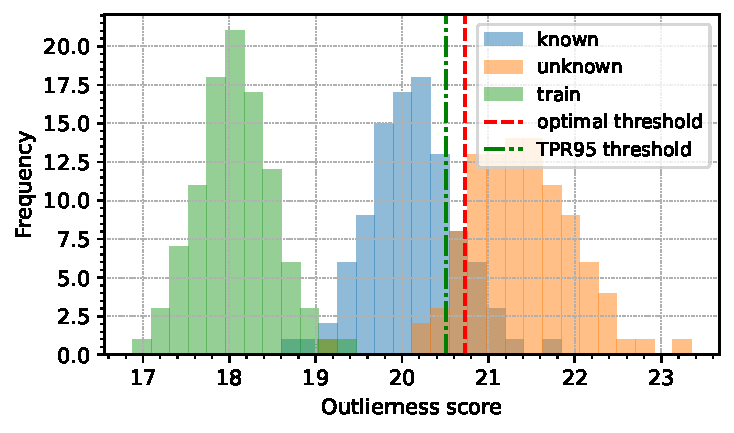
\includegraphics[width=\textwidth]{images/distributions/histograms/hist-distributions-dimension_250-samples_1000-distance_8-distribution_gaussian-model_kNN-10-seed_0.pdf}
        \label{fig:histogram-knn}
    \end{subfigure}
    \begin{subfigure}[b]{0.495\textwidth}
        \centering
        \caption{\small Local Outlier Factor ($k=10$)}
        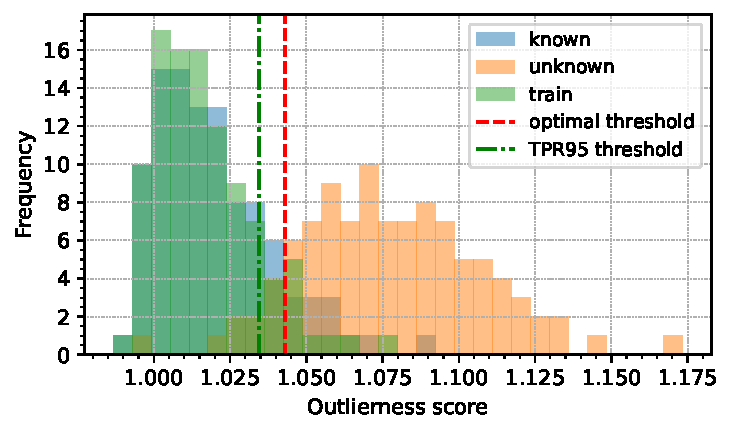
\includegraphics[width=\textwidth]{images/distributions/histograms/hist-distributions-dimension_250-samples_1000-distance_8-distribution_gaussian-model_LOF-10-seed_0.pdf}
        \label{fig:histogram-lof}
    \end{subfigure}
    \hfill
    \begin{subfigure}[b]{0.495\textwidth}
        \centering
        \caption{\small Mahalanobis distance}
        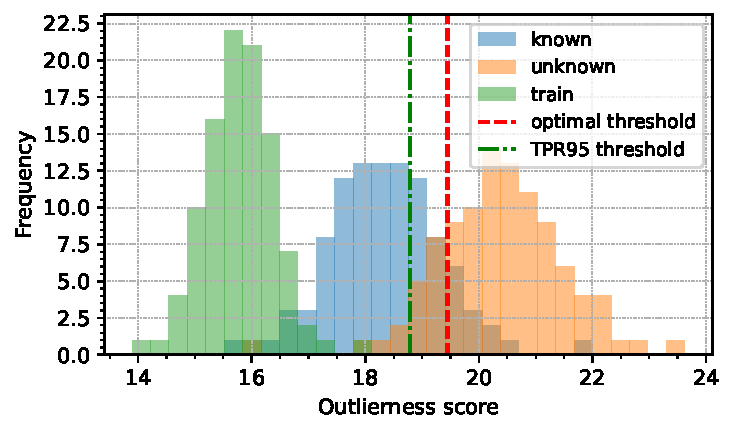
\includegraphics[width=\textwidth]{images/distributions/histograms/hist-distributions-dimension_250-samples_1000-distance_8-distribution_gaussian-model_MD-seed_0.pdf}
        \label{fig:histogram-mahalanobis}
    \end{subfigure}
    \caption{The distributions of outlierness scores obtained for various $OF$ measures (ABOF, ED, IRWD, kNN, LOF, MD). For all cases the same configuration of $T$, $K$ and $U$ clusters is~used – containing $n = 1000$ training samples, dimension of feature vectors $d = 250$, generated from $G = \textit{Gaussian}$ distribution, seed $\xi = 0$; outliers are shifted by~distance $h = 8$. In~some cases (kNN, MD) the results obtained for $K$ are~surprisingly~distant from results obtained for $T$.}
    \label{fig:histograms}
\end{figure}

\begin{figure}[t]
    % StreamLit settings: width=9, height=2
    \centering
    \begin{subfigure}[b]{\textwidth}
        \centering
        \caption{\small Angle-Based Outlier Factor}
        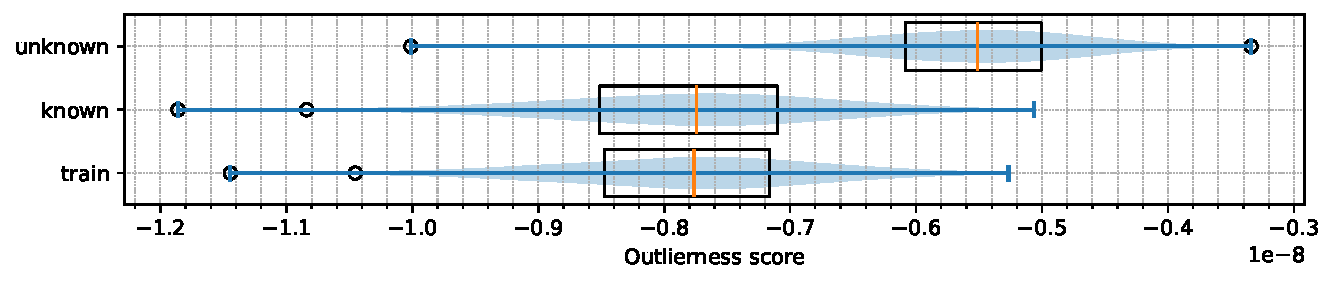
\includegraphics[width=\textwidth]{images/distributions/skew/box-distributions-dimension_250-samples_1000-distance_8-distribution_gaussian-model_ABOF-seed_0.pdf}
        \label{fig:box-abof}
    \end{subfigure}
    \begin{subfigure}[b]{\textwidth}
        \centering
        \caption{\small Euclidean distance}
        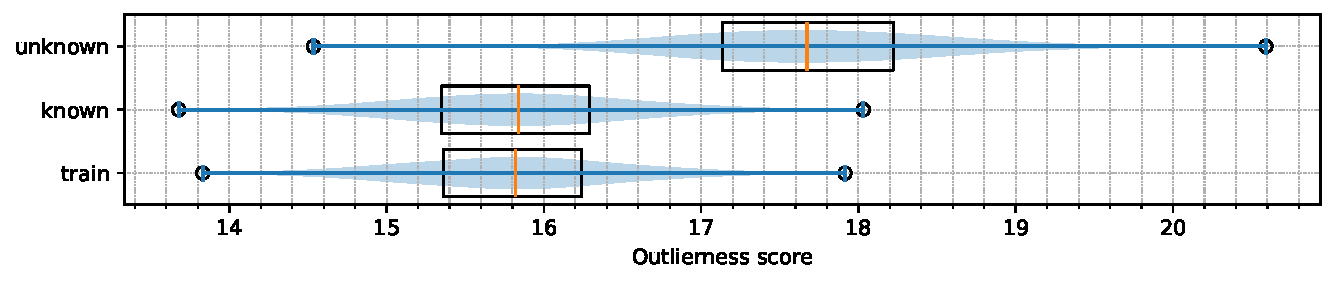
\includegraphics[width=\textwidth]{images/distributions/skew/box-distributions-dimension_250-samples_1000-distance_8-distribution_gaussian-model_ED-seed_0.pdf}
        \label{fig:box-ed}
    \end{subfigure}
    \begin{subfigure}[b]{\textwidth}
        \centering
        \caption{\small k-Nearest Neighbors ($k=10$)}
        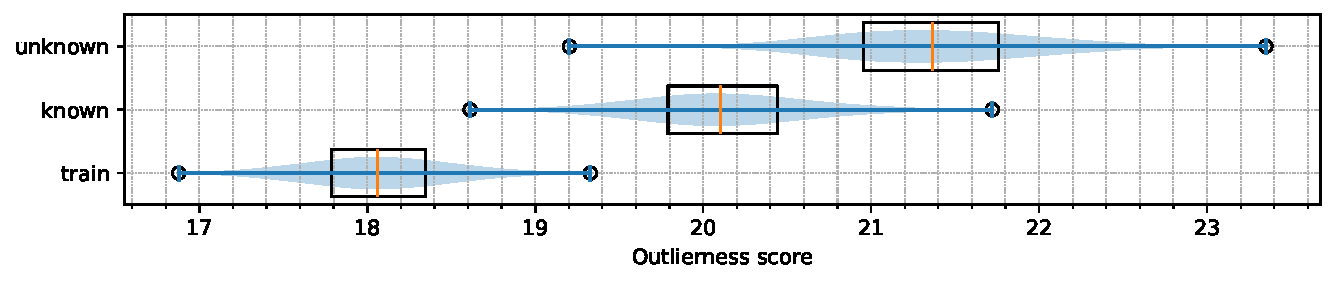
\includegraphics[width=\textwidth]{images/distributions/skew/box-distributions-dimension_250-samples_1000-distance_8-distribution_gaussian-model_kNN-10-seed_0.pdf}
        \label{fig:box-knn}
    \end{subfigure}
    \begin{subfigure}[b]{\textwidth}
        \centering
        \caption{\small Local Outlier Factor ($k=10$)}
        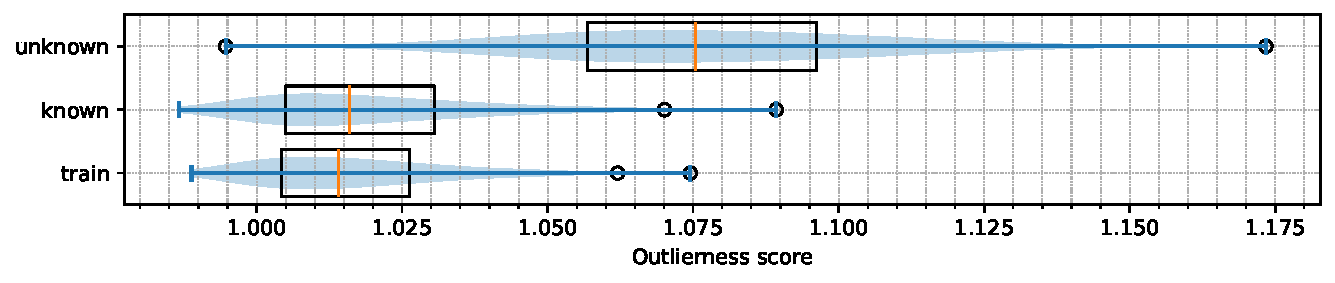
\includegraphics[width=\textwidth]{images/distributions/skew/box-distributions-dimension_250-samples_1000-distance_8-distribution_gaussian-model_LOF-10-seed_0.pdf}
        \label{fig:box-lof}
    \end{subfigure}
    \caption{The boxplots of scores distributions obtained for selected $OF$ measures (ABOF, ED, kNN, LOF) calculated on $T$, $K$ and $U$ clusters – corresponding with selected histograms from the figure \ref{fig:histograms}. The positive skew is observed in case of LOF and negative skew in case of ABOF measure, while ED and kNN appear symmetric.}
    \label{fig:boxplots}
\end{figure}

\begin{figure}[t]
    % StreamLit settings: width=5, height=3
    \centering
    \begin{subfigure}[b]{0.495\textwidth}
        \centering
        \caption{\small k-Nearest Neighbors, $G = \textit{Gaussian}$}
        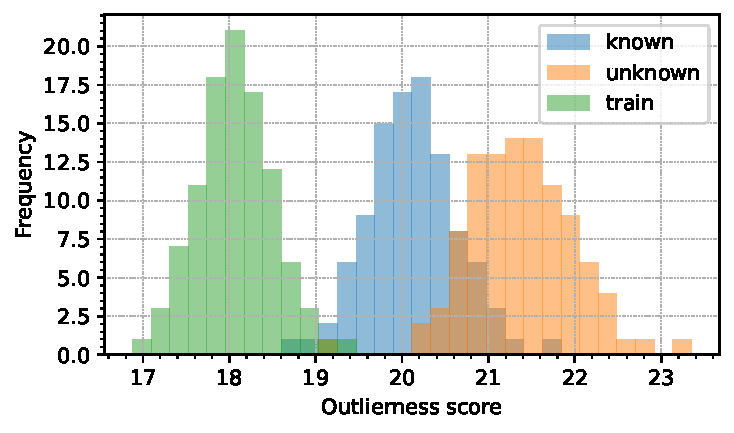
\includegraphics[width=\textwidth]{images/distributions/hists-Gen/hist-distributions-dimension_250-samples_1000-distance_8-distribution_gaussian-model_kNN-10-seed_0.pdf}
        \label{fig:hists-knn-gaussian}
    \end{subfigure}
    \hfill
    \begin{subfigure}[b]{0.495\textwidth}
        \centering
        \caption{\small Mahalanobis distance, $G = \textit{Gaussian}$}
        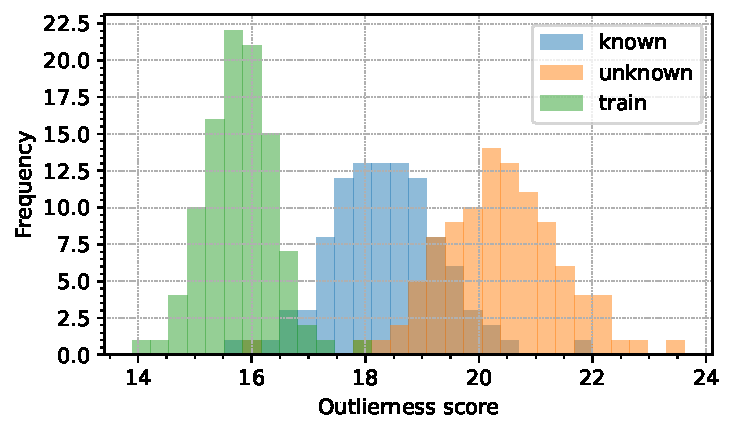
\includegraphics[width=\textwidth]{images/distributions/hists-Gen/hist-distributions-dimension_250-samples_1000-distance_8-distribution_gaussian-model_MD-seed_0.pdf}
        \label{fig:hists-md-gaussian}
    \end{subfigure}
    \begin{subfigure}[b]{0.495\textwidth}
        \centering
        \caption{\small k-Nearest Neighbors, $G = \textit{Triangular}$}
        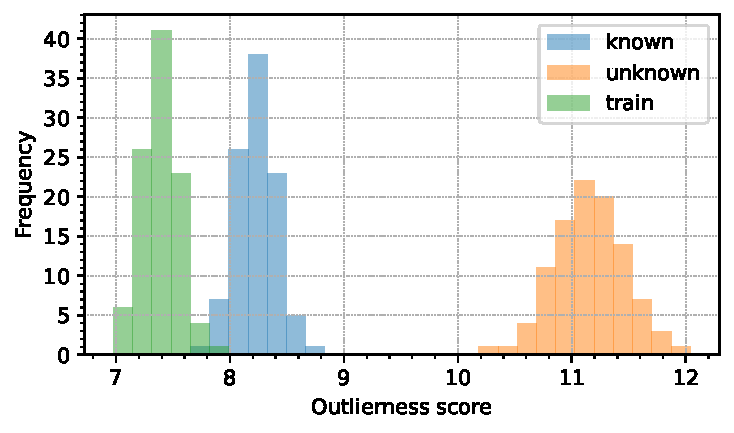
\includegraphics[width=\textwidth]{images/distributions/hists-Gen/hist-distributions-dimension_250-samples_1000-distance_8-distribution_triangular-model_kNN-10-seed_0.pdf}
        \label{fig:hists-knn-triangular}
    \end{subfigure}
    \hfill
    \begin{subfigure}[b]{0.495\textwidth}
        \centering
        \caption{\small Mahalanobis distance, $G = \textit{Triangular}$}
        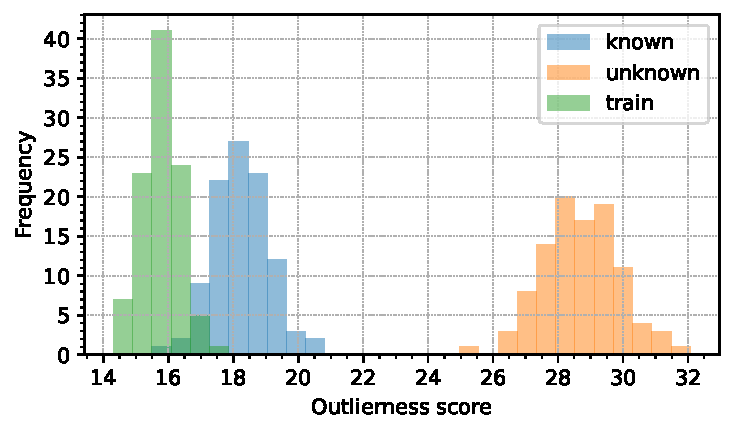
\includegraphics[width=\textwidth]{images/distributions/hists-Gen/hist-distributions-dimension_250-samples_1000-distance_8-distribution_triangular-model_MD-seed_0.pdf}
        \label{fig:hists-md-triangular}
    \end{subfigure}
    \begin{subfigure}[b]{0.495\textwidth}
        \centering
        \caption{\small k-Nearest Neighbors, $G = \textit{Uniform}$}
        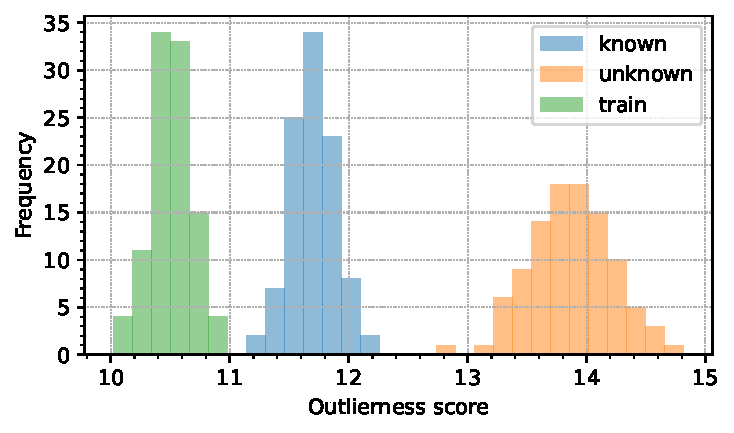
\includegraphics[width=\textwidth]{images/distributions/hists-Gen/hist-distributions-dimension_250-samples_1000-distance_8-distribution_uniform-model_kNN-10-seed_0.pdf}
        \label{fig:hists-knn-uniform}
    \end{subfigure}
    \hfill
    \begin{subfigure}[b]{0.495\textwidth}
        \centering
        \caption{\small Mahalanobis distance, $G = \textit{Uniform}$}
        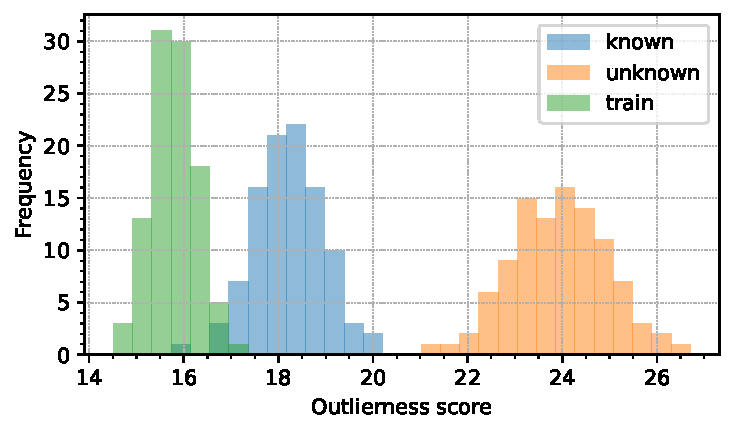
\includegraphics[width=\textwidth]{images/distributions/hists-Gen/hist-distributions-dimension_250-samples_1000-distance_8-distribution_uniform-model_MD-seed_0.pdf}
        \label{fig:hists-md-uniform}
    \end{subfigure}
    \caption{In case of kNN and MD, for high-dimensional feature vectors, the scores for known in-distribution data (cluster $K$) may not overlap with the scores obtained for the training samples (cluster $T$). This phenomenon is observed regardless of~chosen data distribution generator $G$: $\textit{Triangular}$ (shown in figures \ref{fig:hists-knn-triangular} and \ref{fig:hists-md-triangular}) or $\textit{Uniform}$ (figures \ref{fig:hists-knn-uniform} and \ref{fig:hists-md-uniform}) $\textit{Gaussian}$ (figures \ref{fig:histogram-knn} and \ref{fig:histogram-mahalanobis}). Other parameters are the same as for figure \ref{fig:histograms}: $n = 1000$, $d = 250$, $h = 8$, $\xi = 0$.}
    \label{fig:histograms-other-G}
\end{figure}

\begin{figure}[t]
    % StreamLit settings: width=9, height=2
    % Query: model = "MD" and dimension == 250 and 500 <= samples <= 5000 and distance == 8 and seed = 0 and distribution == "uniform"
    \centering
    \begin{subfigure}[b]{\textwidth}
        \centering
        \caption{\small Mahalanobis distance, training samples: $n = 500$}
        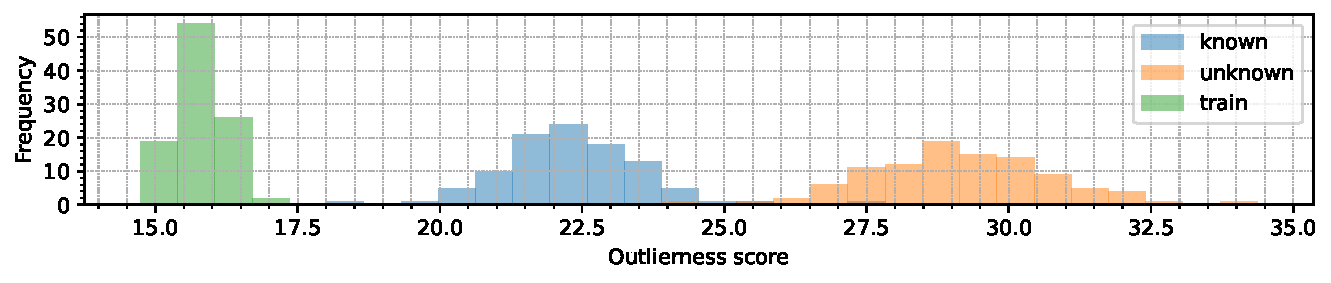
\includegraphics[width=\textwidth]{images/distributions/hists-md-samples/hist-distributions-dimension_250-samples_500-distance_8-distribution_uniform-model_MD-seed_0.pdf}
        \label{fig:hists-md-500}
    \end{subfigure}
    \begin{subfigure}[b]{\textwidth}
        \centering
        \caption{\small Mahalanobis distance, training samples: $n = 1000$}
        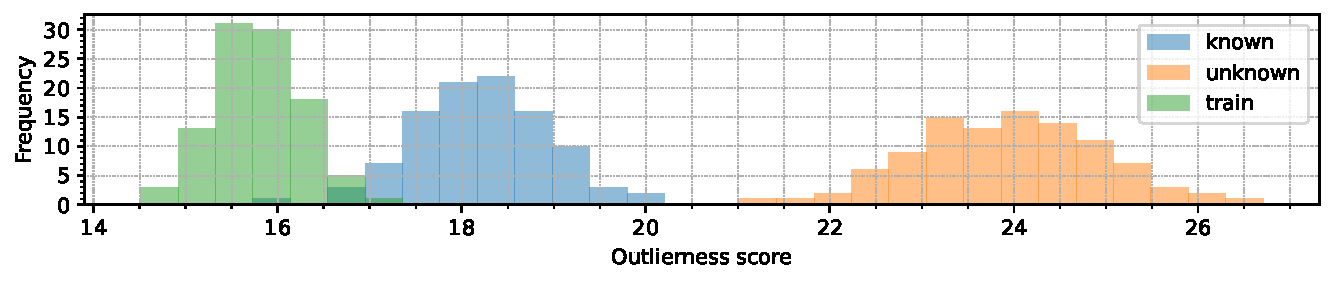
\includegraphics[width=\textwidth]{images/distributions/hists-md-samples/hist-distributions-dimension_250-samples_1000-distance_8-distribution_uniform-model_MD-seed_0.pdf}
        \label{fig:hists-md-1000}
    \end{subfigure}
    \begin{subfigure}[b]{\textwidth}
        \centering
        \caption{\small Mahalanobis distance, training samples: $n = 2500$}
        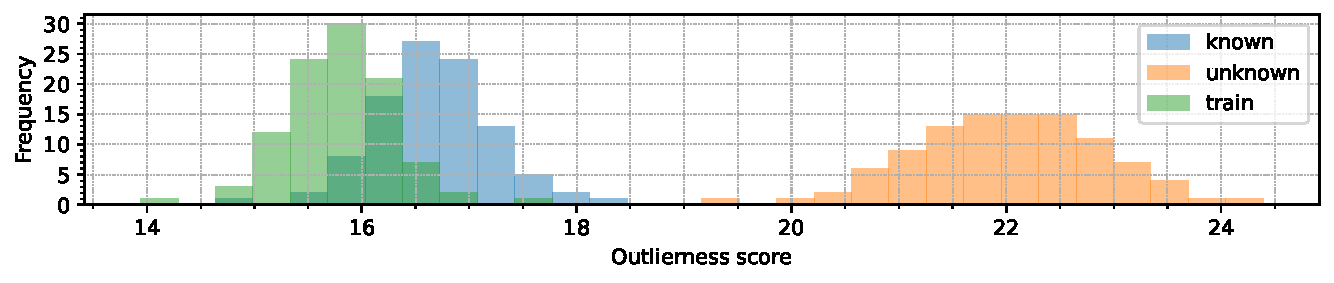
\includegraphics[width=\textwidth]{images/distributions/hists-md-samples/hist-distributions-dimension_250-samples_2500-distance_8-distribution_uniform-model_MD-seed_0.pdf}
        \label{fig:hists-md-2500}
    \end{subfigure}
    \begin{subfigure}[b]{\textwidth}
        \centering
        \caption{\small Mahalanobis distance, training samples: $n = 5000$}
        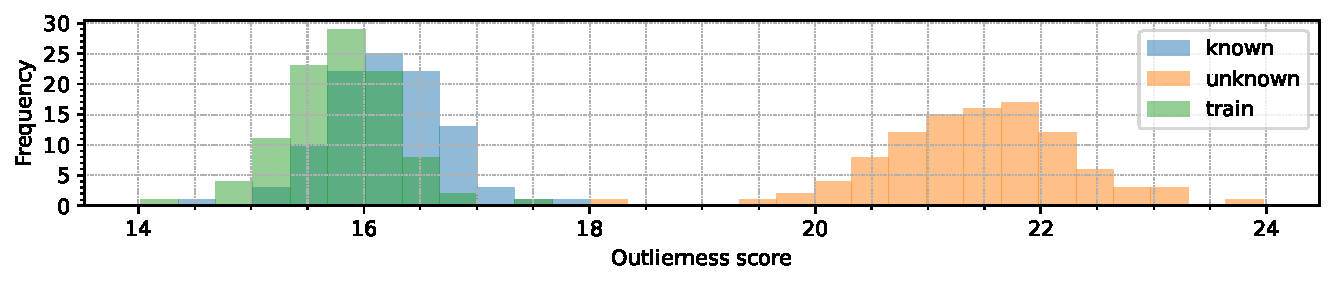
\includegraphics[width=\textwidth]{images/distributions/hists-md-samples/hist-distributions-dimension_250-samples_5000-distance_8-distribution_uniform-model_MD-seed_0.pdf}
        \label{fig:hists-md-5000}
    \end{subfigure}
    \caption{The distance between scores for known data (in-distribution, cluster $K$) and training examples (cluster $T$) gets smaller for MD when the training cluster $T$ contains more elements (parameter $n$). Note that the outliers (unknown examples, cluster $U$) are also moving closer to~$T$ (distances between medians $Q2_{T}$ and $Q2_{U}$: $\Delta{Q}_{n=500} \approx 13.31$ $\rightarrow$ $\Delta{Q}_{n=1000} \approx 8.19$ $\rightarrow$ $\Delta{Q}_{n=2500} \approx 6.22$ $\rightarrow$ $\Delta{Q}_{n=5000} \approx 5.68$), \\
    up to a~certain point –~when $K$ overlaps with $T$, then cluster $U$ no longer moves towards cluster $T$. Other distribution parameters involved: \\
    $d = 250$, $h = 8$, $G = \textit{Uniform}$, $\xi = 0$.}
    \label{fig:hists-md-samples}
\end{figure}

\begin{figure}[t]
    % StreamLit settings: width=9, height=2
    \centering
    \begin{subfigure}[b]{\textwidth}
        \centering
        \caption{\small k-Nearest Neighbors ($k=10$), training samples: $n = 500$}
        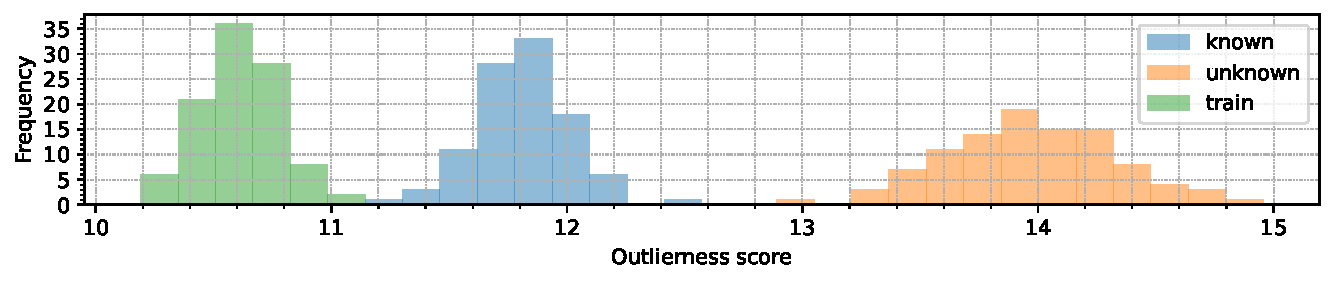
\includegraphics[width=\textwidth]{images/distributions/hists-knn-samples/hist-distributions-dimension_250-samples_500-distance_8-distribution_uniform-model_kNN-10-seed_0.pdf}
        \label{fig:hists-knn-500}
    \end{subfigure}
    \begin{subfigure}[b]{\textwidth}
        \centering
        \caption{\small k-Nearest Neighbors ($k=10$), training samples: $n = 1000$}
        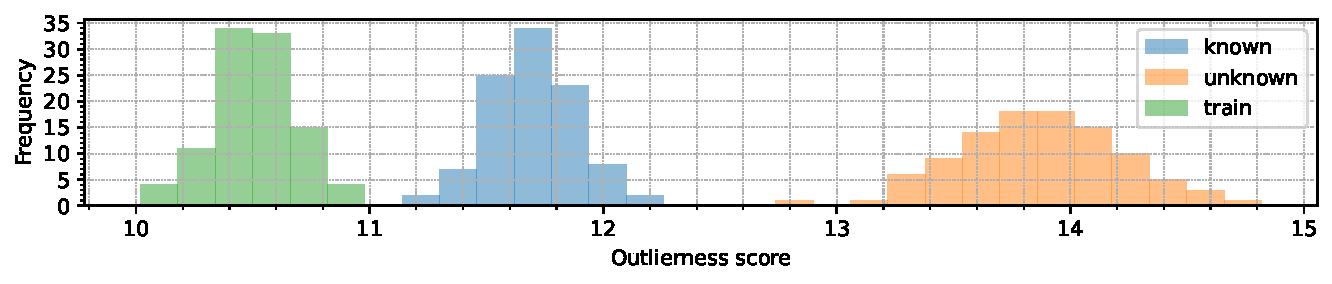
\includegraphics[width=\textwidth]{images/distributions/hists-knn-samples/hist-distributions-dimension_250-samples_1000-distance_8-distribution_uniform-model_kNN-10-seed_0.pdf}
        \label{fig:hists-knn-1000}
    \end{subfigure}
    \begin{subfigure}[b]{\textwidth}
        \centering
        \caption{\small k-Nearest Neighbors ($k=10$), training samples: $n = 5000$}
        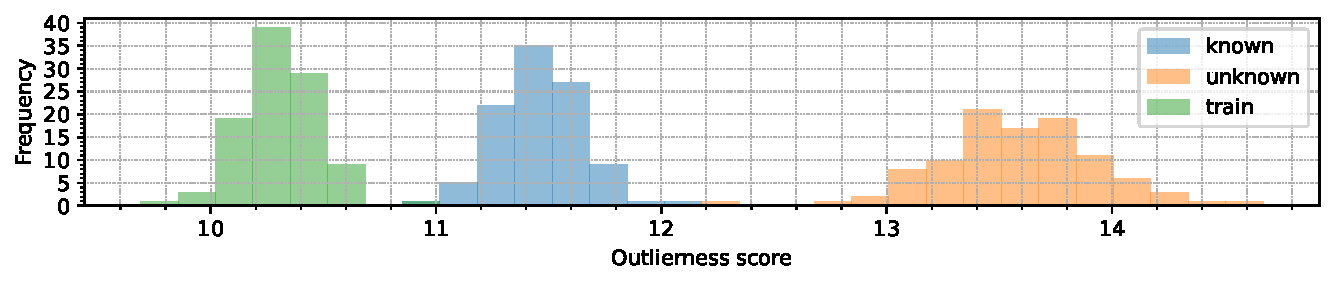
\includegraphics[width=\textwidth]{images/distributions/hists-knn-samples/hist-distributions-dimension_250-samples_5000-distance_8-distribution_uniform-model_kNN-10-seed_0.pdf}
        \label{fig:hists-knn-5000}
    \end{subfigure}
    \begin{subfigure}[b]{\textwidth}
        \centering
        \caption{\small k-Nearest Neighbors ($k=20$), training samples: $n = 1000$}
        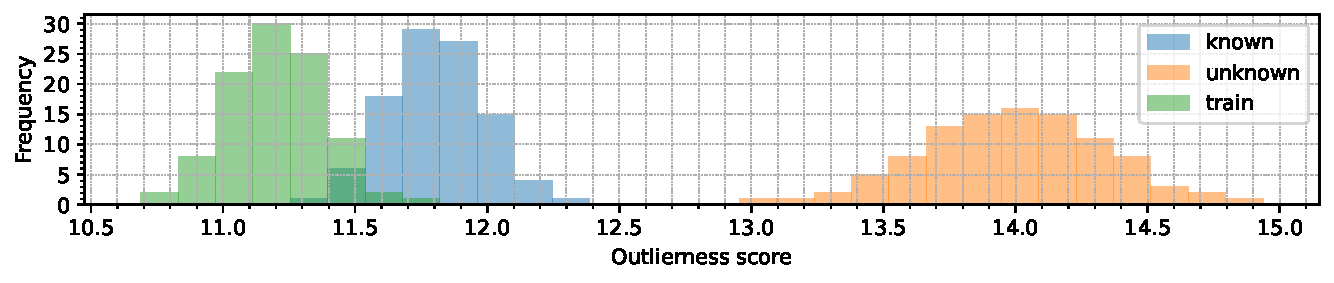
\includegraphics[width=\textwidth]{images/distributions/hists-knn-samples/hist-distributions-dimension_250-samples_1000-distance_8-distribution_uniform-model_kNN-20-seed_0.pdf}
        \label{fig:hists-knn20-1000}
    \end{subfigure}
    \caption{Unlike for MD, increasing the number of training samples $n$ in cluster $T$ does not bring the cluster $K$ scores significantly closer to scores for cluster $T$. Scores obtained for outliers (cluster $U$) also remain unaffected by $n$. However, the results for~$K$ and $T$ start to overlap for larger values of $k$ (parameter of kNN algorithm). Experiment settings are the same as in figure \ref{fig:hists-md-samples} ({\small$d = 250$, $h = 8$, $G = \textit{Uniform}$, $\xi = 0$}).}
    \label{fig:hists-knn-samples}
\end{figure}

\begin{figure}[t]
    % StreamLit settings: width=9, height=2
    \centering
    \begin{subfigure}[b]{\textwidth}
        \centering
        \caption{\small k-Nearest Neighbors ($k=10$), dimension of feature vectors: $d = 100$}
        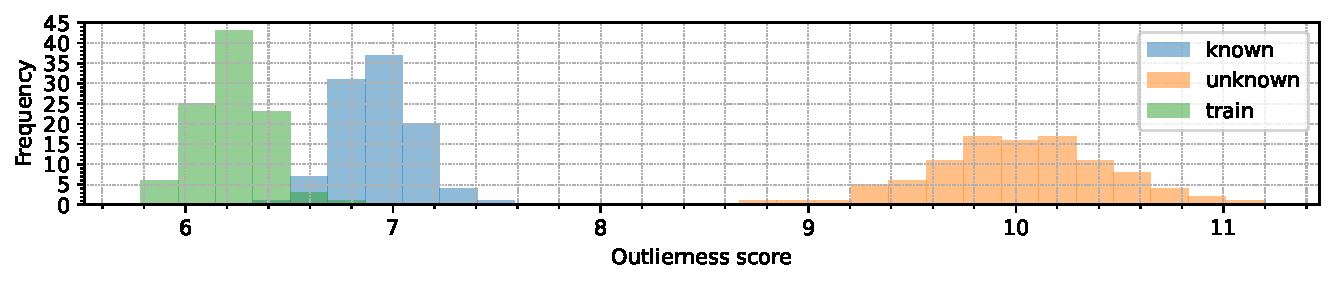
\includegraphics[width=\textwidth]{images/distributions/hists-dimensions/hist-distributions-dimension_100-samples_1000-distance_8-distribution_uniform-model_kNN-10-seed_0.pdf}
        \label{fig:hists-knn-d100}
    \end{subfigure}
    \begin{subfigure}[b]{\textwidth}
        \centering
        \caption{\small k-Nearest Neighbors ($k=10$), dimension of feature vectors: $d = 500$}
        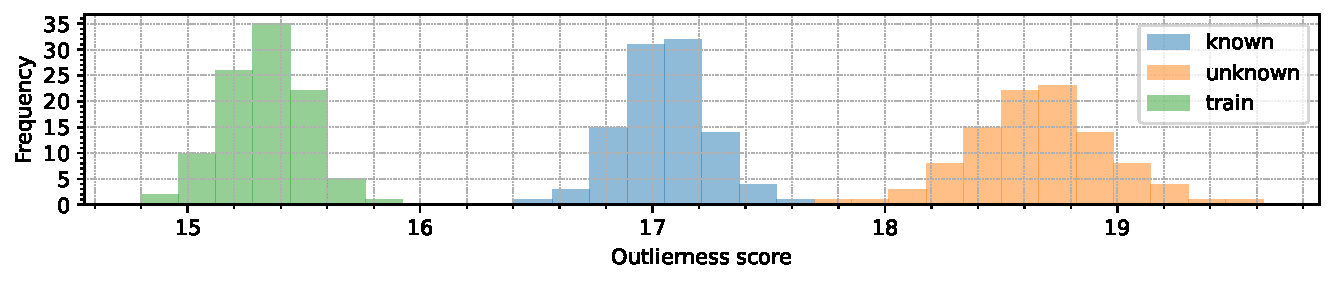
\includegraphics[width=\textwidth]{images/distributions/hists-dimensions/hist-distributions-dimension_500-samples_1000-distance_8-distribution_uniform-model_kNN-10-seed_0.pdf}
        \label{fig:hists-knn-d500}
    \end{subfigure}
    \begin{subfigure}[b]{\textwidth}
        \centering
        \caption{\small Mahalanobis distance, dimension of feature vectors: $d = 100$}
        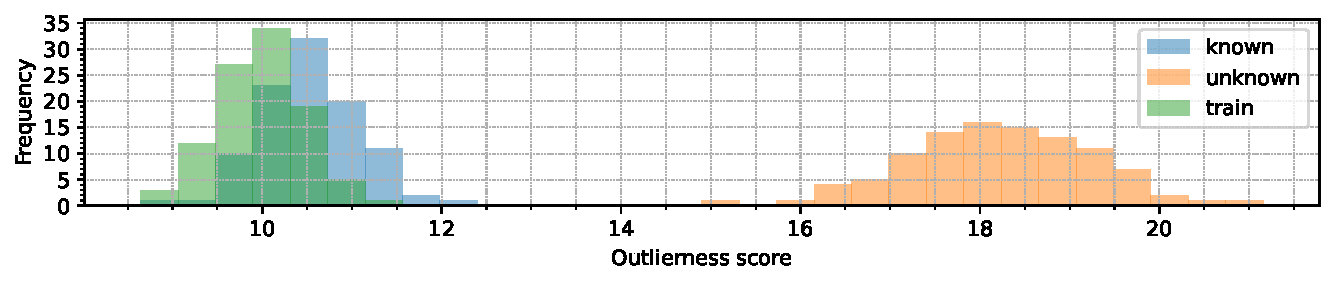
\includegraphics[width=\textwidth]{images/distributions/hists-dimensions/hist-distributions-dimension_100-samples_1000-distance_8-distribution_uniform-model_MD-seed_0.pdf}
        \label{fig:hists-md-d100}
    \end{subfigure}
    \begin{subfigure}[b]{\textwidth}
        \centering
        \caption{\small Mahalanobis distance, dimension of feature vectors: $d = 500$}
        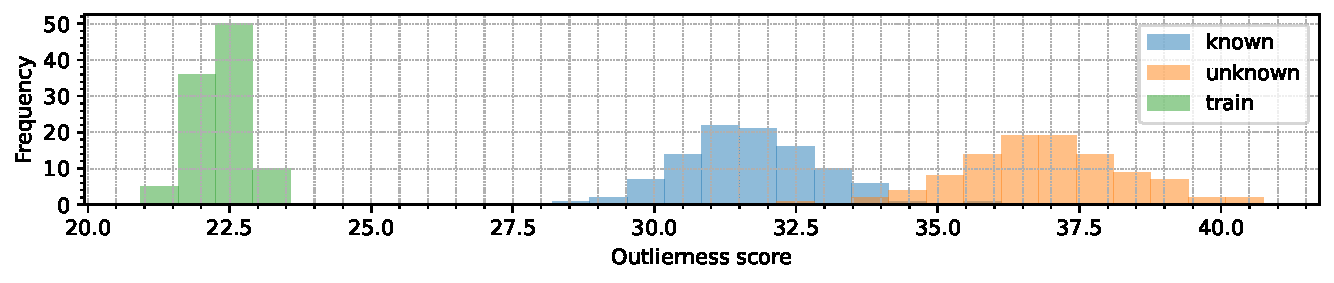
\includegraphics[width=\textwidth]{images/distributions/hists-dimensions/hist-distributions-dimension_500-samples_1000-distance_8-distribution_uniform-model_MD-seed_0.pdf}
        \label{fig:hists-md-d500}
    \end{subfigure}
    \caption{The effect of distancing scores acquired for cluster $K$ from the scores obtained for cluster $T$, observed in case of kNN and MD measures, is stronger for increased dimensionality of feature vectors $d$. It can be noticed that for higher dimensions the scores values are also greater, as both the measures are based on spatial distances in features space, hence more feature vectors components contribute to~greater score values. Results visible in plots are obtained for experiment settings: $n = 1000$, $h = 8$, $G = \textit{Uniform}$, $\xi = 0$.}
    \label{fig:hists-dimensions}
\end{figure}

\begin{figure}[tb]
    \vspace{-2.0em}
    % StreamLit settings: width=9, height=2
    \centering
    \begin{subfigure}[b]{\textwidth}
        \centering
        \caption{\small Standardized Euclidean distance, dimension of feature vectors: $d = 100$}
        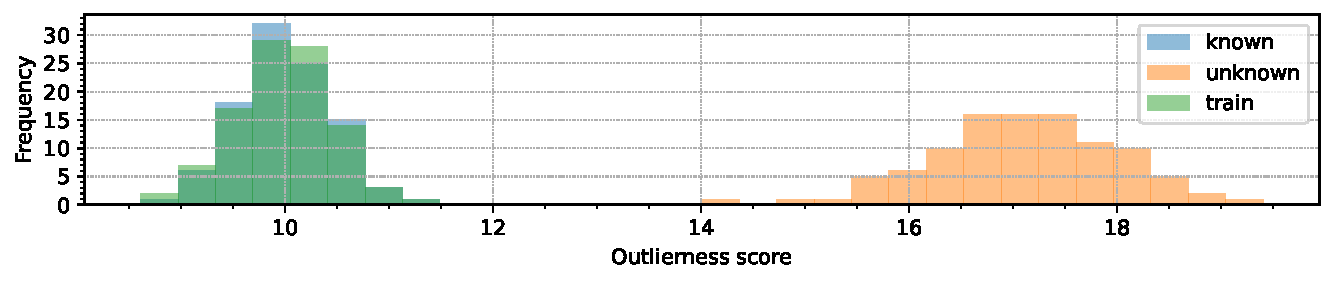
\includegraphics[width=\textwidth]{images/distributions/hists-sed-dimensions/hist-distributions-dimension_100-samples_1000-distance_8-distribution_uniform-model_SED-seed_0.pdf}
        \label{fig:hists-sed-100}
    \end{subfigure}
    \begin{subfigure}[b]{\textwidth}
        \centering
        \caption{\small Standardized Euclidean distance, dimension of feature vectors: $d = 500$}
        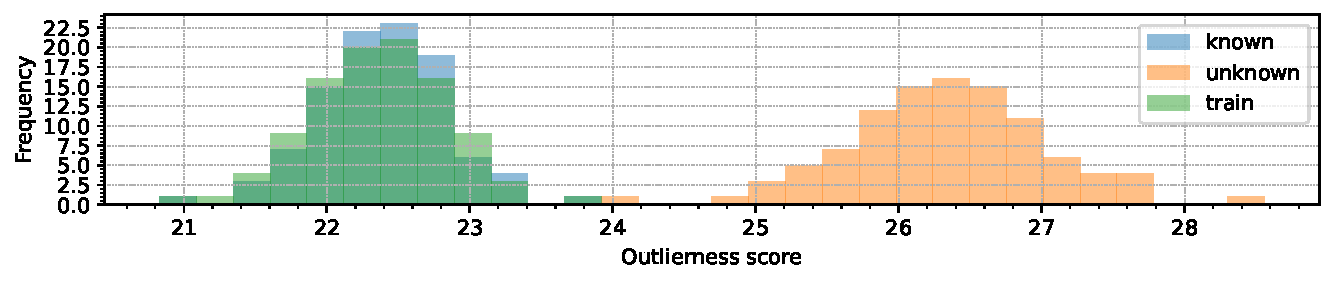
\includegraphics[width=\textwidth]{images/distributions/hists-sed-dimensions/hist-distributions-dimension_500-samples_1000-distance_8-distribution_uniform-model_SED-seed_0.pdf}
        \label{fig:hists-sed-500}
    \end{subfigure}
    \caption{For measures ABOF, IRWD, LOF, ED and SED, in typical conditions, $n \gtrsim d$, the separation between scores for in-distribution data (cluster $K$ and cluster $T$) is not observed, maintaining good overlapping even for a lower number of training samples $n$ than for MD. Experiment settings: $n = 1000$, $h = 8$, $G = \textit{Uniform}$, $\xi = 0$.}
    \label{fig:hists-sed-dimensions}
\end{figure}
\begin{figure}[tb]
    \vspace{-1.0em}
    % StreamLit settings: width=9, height=2
    \centering
    \begin{subfigure}[b]{\textwidth}
        \centering
        \caption{\small Angle-Based Outlier Factor, dimension: $d = 1000$, samples: $n = 50$}
        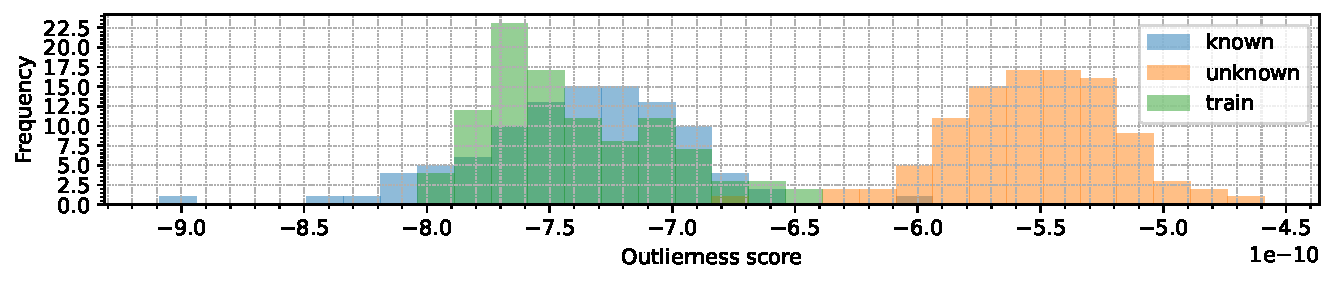
\includegraphics[width=\textwidth]{images/distributions/hists-extreme/hist-distributions-dimension_1000-samples_50-distance_8-distribution_uniform-model_ABOF-seed_0.pdf}
        \label{fig:hists-abof-n50}
    \end{subfigure}
    \begin{subfigure}[b]{\textwidth}
        \centering
        \caption{\small Local Outlier Factor ($k=10$), dimension: $d = 1000$, samples: $n = 50$}
        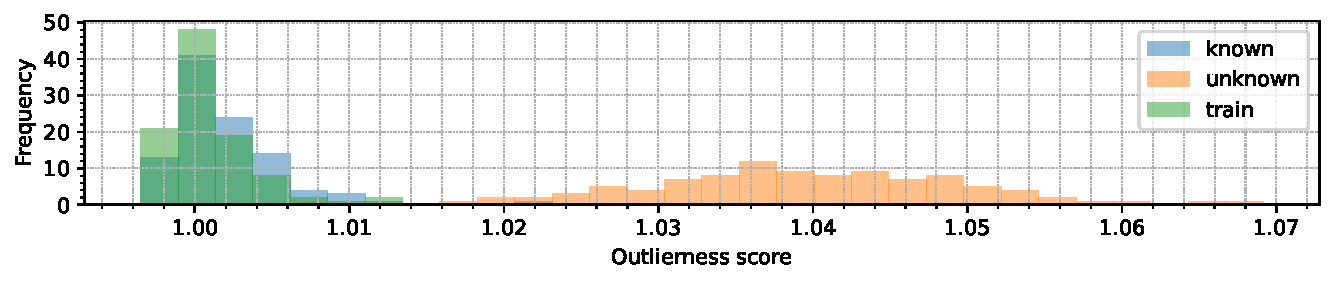
\includegraphics[width=\textwidth]{images/distributions/hists-extreme/hist-distributions-dimension_1000-samples_50-distance_8-distribution_uniform-model_LOF-10-seed_0.pdf}
        \label{fig:hists-lof-n50}
    \end{subfigure}
    \caption{In the performed study, ABOF and LOF were able to produce accurate representations even in case of significantly under-represented testing cluster –~obtained scores for $T$ and $K$ do overlap despite $n = 50$ training samples for $d = 1000$ dimension of feature vectors. Remaining experiment settings are: $h = 8$, $G = \textit{Uniform}$, $\xi = 0$.}
    \label{fig:hists-extreme-good}
    \vspace{-3.0em}
\end{figure}

\begin{figure}[t]
    % StreamLit settings: width=9, height=2
    \centering
    \begin{subfigure}[b]{\textwidth}
        \centering
        \caption{\small Integrated Rank Weighted Depth ({\scriptsize$n_{proj} = 10^3$}), dimension: $d = 500$, samples: $n = 50$}
        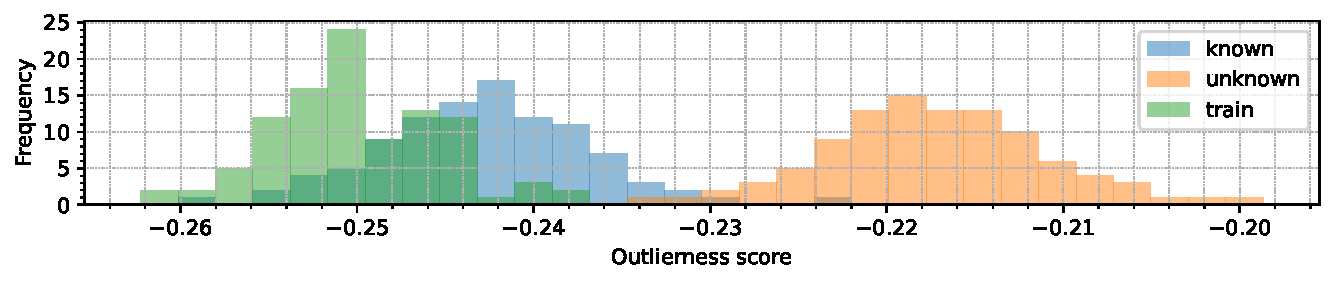
\includegraphics[width=\textwidth]{images/distributions/hists-extreme/hist-distributions-dimension_500-samples_50-distance_8-distribution_uniform-model_IRWD-1000-seed_0.pdf}
        \label{fig:hists-irwd-n50}
    \end{subfigure}
    \begin{subfigure}[b]{\textwidth}
        \centering
        \caption{\small Integrated Rank Weighted Depth ({\scriptsize$n_{proj} = 10^3$}), dimension: $d = 500$, samples: $n = 500$}
        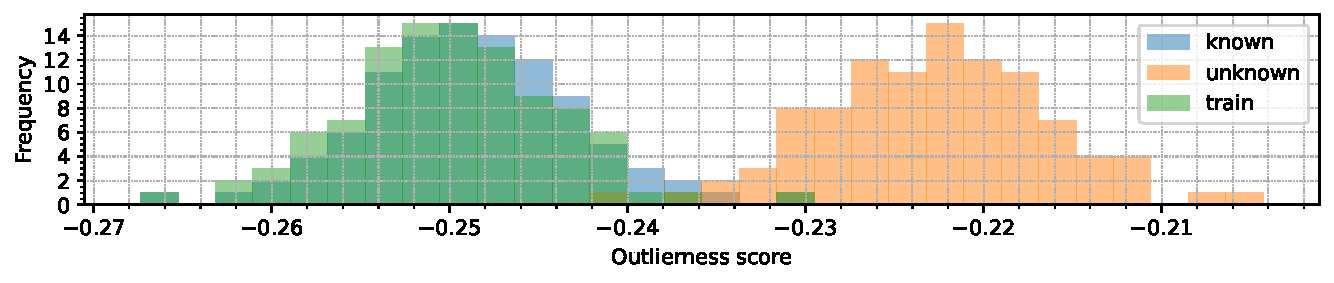
\includegraphics[width=\textwidth]{images/distributions/hists-extreme/hist-distributions-dimension_500-samples_500-distance_8-distribution_uniform-model_IRWD-1000-seed_0.pdf}
        \label{fig:hists-irwd-n500}
    \end{subfigure}
    \begin{subfigure}[b]{\textwidth}
        \centering
        \caption{\small Standardized Euclidean distance, dimension: $d = 1000$, training samples: $n = 50$}
        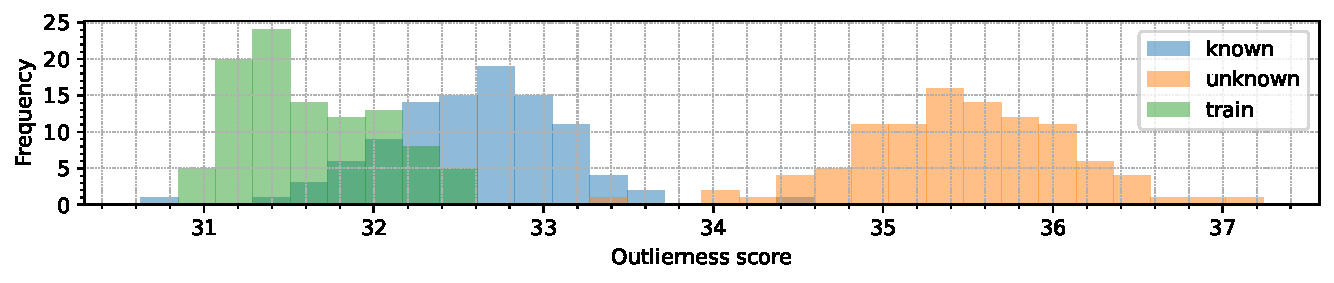
\includegraphics[width=\textwidth]{images/distributions/hists-extreme/hist-distributions-dimension_1000-samples_50-distance_8-distribution_uniform-model_SED-seed_0.pdf}
        \label{fig:hists-sed-n50}
    \end{subfigure}
    \begin{subfigure}[b]{\textwidth}
        \centering
        \caption{\small Standardized Euclidean distance, dimension: $d = 1000$, training samples: $n = 1000$}
        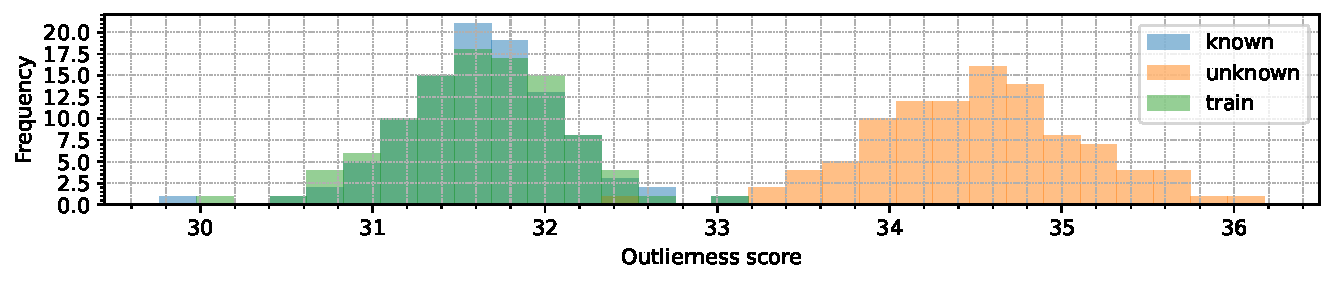
\includegraphics[width=\textwidth]{images/distributions/hists-extreme/hist-distributions-dimension_1000-samples_1000-distance_8-distribution_uniform-model_SED-seed_0.pdf}
        \label{fig:hists-sed-n1000}
    \end{subfigure}
    \caption{For strongly under-represented training clusters, $n \ll d$, the effect of~not-overlapping between the scores for cluster $T$ and $K$ is observed in case of~IRWD, ED and SED measures. The effect vanishes when $n$ is not so low, yet it does not need to be as big as for MD to reach overlapping (settings: $h = 8$, $G = \textit{Uniform}$, $\xi = 0$).}
    \label{fig:hists-extreme-bad}
\end{figure}

\begin{figure}[t]
    % StreamLit settings: width=5, height=3
    \centering
    \begin{subfigure}[b]{0.495\textwidth}
        \centering
        \caption{\small Angle-Based Outlier Factor}
        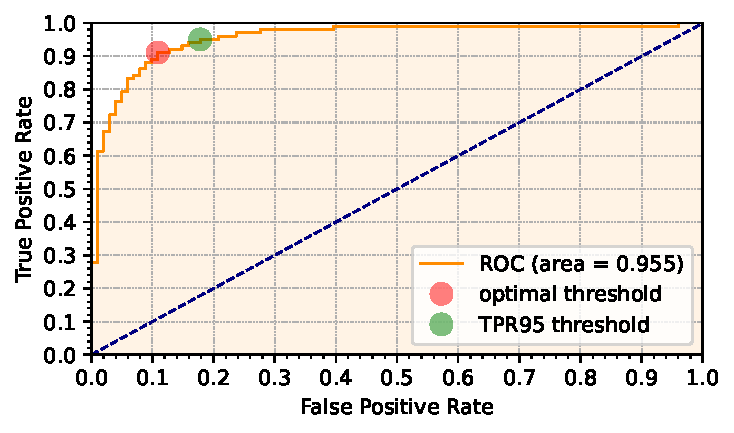
\includegraphics[width=\textwidth]{images/distributions/rocs/roc-distributions-dimension_250-samples_1000-distance_8-distribution_gaussian-model_ABOF-seed_0.pdf}
        \label{fig:roc-abof}
    \end{subfigure}
    \hfill
    \begin{subfigure}[b]{0.495\textwidth}
        \centering
        \caption{\small Euclidean distance}
        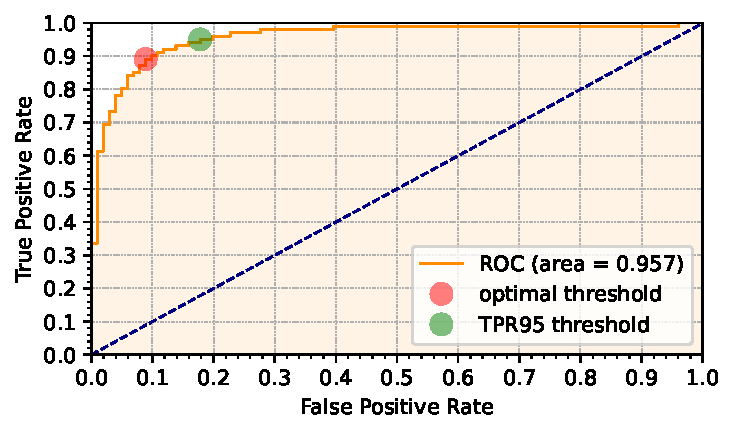
\includegraphics[width=\textwidth]{images/distributions/rocs/roc-distributions-dimension_250-samples_1000-distance_8-distribution_gaussian-model_ED-seed_0.pdf}
        \label{fig:roc-euclidean}
    \end{subfigure}
    \begin{subfigure}[b]{0.495\textwidth}
        \centering
        \caption{\footnotesize Integrated Rank Weighted Depth ({\scriptsize$n_{proj} = 10^3$})}
        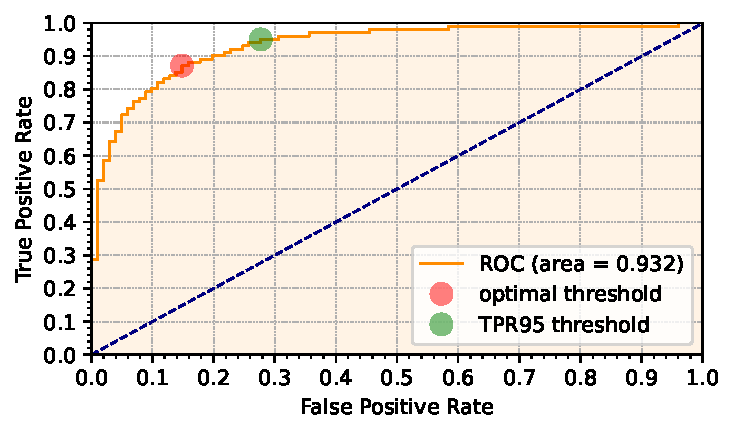
\includegraphics[width=\textwidth]{images/distributions/rocs/roc-distributions-dimension_250-samples_1000-distance_8-distribution_gaussian-model_IRWD-1000-seed_0.pdf}
        \label{fig:roc-irwd}
    \end{subfigure}
    \hfill
    \begin{subfigure}[b]{0.495\textwidth}
        \centering
        \caption{\small k-Nearest Neighbors ($k=10$)}
        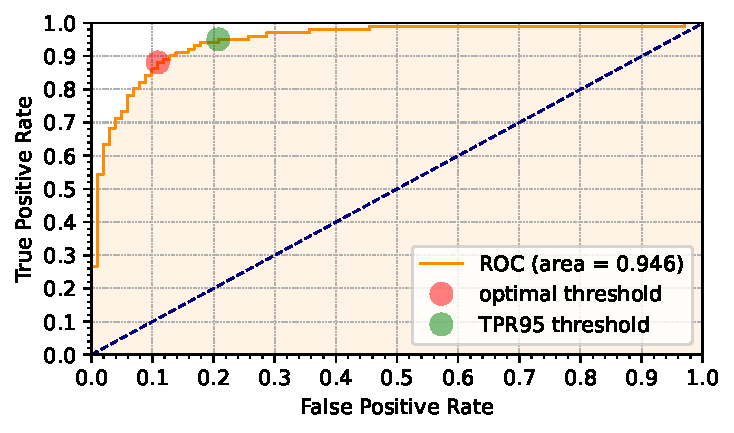
\includegraphics[width=\textwidth]{images/distributions/rocs/roc-distributions-dimension_250-samples_1000-distance_8-distribution_gaussian-model_kNN-10-seed_0.pdf}
        \label{fig:roc-knn}
    \end{subfigure}
    \begin{subfigure}[b]{0.495\textwidth}
        \centering
        \caption{\small Local Outlier Factor ($k=10$)}
        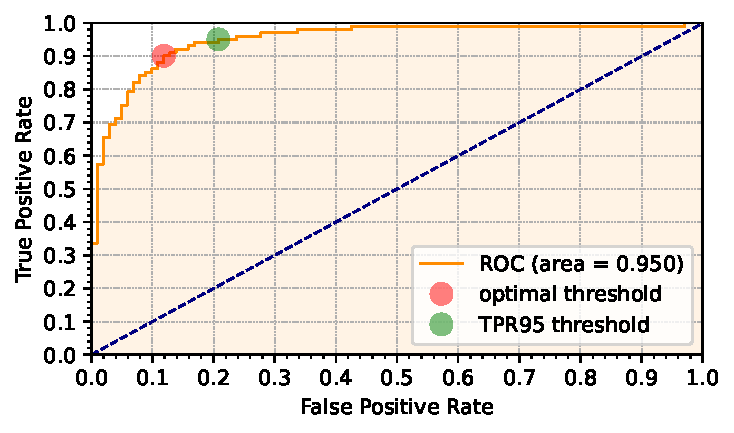
\includegraphics[width=\textwidth]{images/distributions/rocs/roc-distributions-dimension_250-samples_1000-distance_8-distribution_gaussian-model_LOF-10-seed_0.pdf}
        \label{fig:roc-lof}
    \end{subfigure}
    \hfill
    \begin{subfigure}[b]{0.495\textwidth}
        \centering
        \caption{\small Mahalanobis distance}
        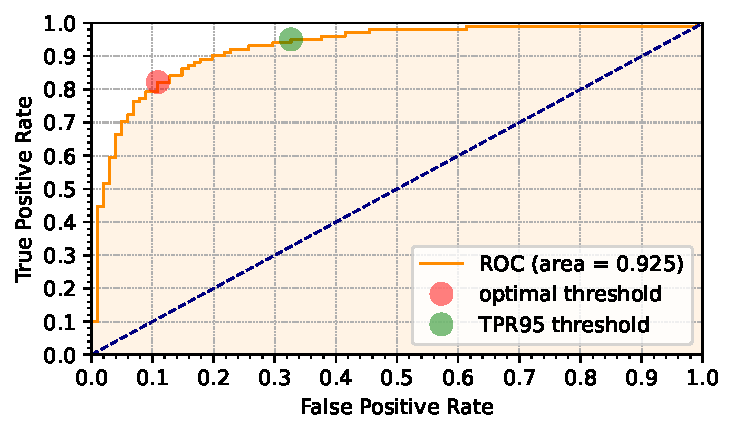
\includegraphics[width=\textwidth]{images/distributions/rocs/roc-distributions-dimension_250-samples_1000-distance_8-distribution_gaussian-model_MD-seed_0.pdf}
        \label{fig:roc-mahalanobis}
    \end{subfigure}
    \caption{The Receiver Operating Characteristic (ROC) curves obtained for various $OF$ measures (ABOF, ED, IRWD, kNN, LOF, MD). They show the sepearability between clusters $K$ and $U$ visible in corresponding plots from the~figure~\ref{fig:histograms}.
    Despite that some $OF$ methods represent $K$ as distant from $T$, they still can distinguish between $K$ and $U$ quite well, all acquiring high AUROC scores \\
    (the~area values of visible subplots are all greater than $0.9$).}
    \label{fig:rocs}
\end{figure}

\cleardoublepage{}

\subsection{Experiment results – effects of parameters}
\label{section:distributions-results-trends}

Figure \ref{fig:dimension} illustrates how the performance of outlierness measures is affected by the dimension of the feature vectors $d$, under fixed number of training samples $n = 2500$ and distance to outliers $h = 8$. The experiments shows that higher the feature space dimension $d$, the more challenging the comparison between data vectors is, as both classification accuracy and AUROC score decrease. The research was focused on ED, IRWD, kNN, LOF, MD and SED measures, omitting ABOF as computationally too expensive and impractical for usage (primarily due to $n$; although it was reaching promising top-scores for lower $n$ and $d$).

All of the analyzed measures $OF$ provide good separability of in-distribution data and outliers in lower dimensions – reaching AUROC value above $0.95$ for $d \leq 200$. In higher dimensions, the outliers distribution appear closer to the training data, so the obtained AUROC values are lower, decreasing exponentially with $d$. For dimension $d = 1000$ the AUROC reaches about ${\sim}0.85$ in case of ED and SED (plots overlap in figure \ref{fig:dimension-auroc}), ${\sim}0.84$ for kNN and LOF, ${\sim}0.78$ for MD and ${\sim}0.715$ in case of IRWD (results visible in subfigure \ref{fig:dimension-auroc}).

Although offering good separability, when the measures are involved in the classification task with respect to the training data only, not all $OF$s perform so well. Notably the kNN's performance falls drastically, reaching accuracy of ${\sim}0.5$ for $d \geq 250$. Similarly, the MD measure, after initially performing well ($d \leq 250$), shows gradual decay of accuracy in higher dimensions ($d \geq 500$). In both mentioned cases it is related to the lose of sensitivity, as visible in figure \ref{fig:dimension-sensitivity} – at some point all in-distribution data were recognized as outliers by kNN and MD (due to the same effect discussed in previous subsection \ref{section:distributions-results-properties} and visible in figure \ref{fig:hists-dimensions}).
% This is significant because, in the real-world scenario, where we would not know where the outliers are distributed, our OOD detection threshold should only rely on the distribution of the available training set. However, as shown in this example, this may lead to poor classification accuracy, as accuracy finally drops to 50\% (i.e., all data are classified as outliers).
% TODO \todo{significant}

Contrary, in case of ED, SED, IRWD and LOF the lowered accuracy in high-dimensions is related purely to the decaying specificity – some out-of-distribution data are seen as too close to the training data, such as in histograms in previous subsection \ref{section:distributions-results-properties} (subfigures \ref{fig:histogram-euclidean}, \ref{fig:histogram-irwd} and \ref{fig:histogram-lof}), hence spuriously considered as inliers.

Figure \ref{fig:samples} shows analogous research, analyzing the performance of outlierness measures $OF$ affected by the number of training samples $n$, having fixed dimension of the feature vectors $d = 750$ and distance to outliers $h = 8$. Surprisingly, no strong influence between the accuracy and separability (AUROC value) is observed – except for extremely underrepresented cases ($n < 100$ for $d = 750$, not show in the figure) or~Mahalanobis Distance measure.

The estimation of covariance matrix for MD in features space of dimension $d = 750$ requires at least $n \geq 750$ data samples. Hence, first reasonable result for MD visible in figure \ref{fig:samples-auroc} appears for $n = 1000$ –~AUROC value ${\sim}0.715$; for $n = 750$ samples the AUROC is ${\sim}0.5$. For $n = 10000$ samples the reaches close to top AUROC score ${\sim}0.85$.

The best separability in analyzed case is again observed for ED and SED measures (AUROC values ${\sim}0.86$), then kNN and LOF (AUROC values ${\sim}0.85$). The IRWD performed significantly worse, scoring AUROC value ${\sim}0.76$. Similarly like in previously examined case, the good AUROC score does not translate to good accuracy in the classification task with respect to the training data. Again, it is due to the zero TPR score (sensitivity) – all in-distribution data are incorrectly recognized as outliers, because the outlierness scores for testing set do not overlap the scores for training set (as visible in figure \ref{fig:hists-dimensions}). In case of MD, low accuracy is observed for up to $n \leq 2500$ samples, because of the same effect as for kNN, however by providing more training samples ($n \geq 5000$) the scores for in-distribution testing samples start to overlap with scores for training samples (effect visible in figure \ref{fig:hists-md-samples}), in the end obtaining one of the top accuracy for $n = 10000$. Yet, ED, SED and LOF reach similar accuracy for lower number of training samples $n$.

Finally, figure \ref{fig:distance} presents the performance of outlierness measures $OF$ as affected by the distance to outliers $h$, under fixed dimension of the feature vectors $d = 750$ and number of training samples $n = 2500$. Intuitively, the more distant the outliers are, the easier they are separable and detectable, like discussed in section \ref{section:near-far-ood} (Near OOD vs Far OOD). The relation is analogous as in first analyzed case – resulting in best separability for ED, SED, kNN and LOF, then for MD and worst for IRWD under given experiment configuration. Again, the worst possible accuracy is observed for kNN and MD, as for given $n$ and $d$ all the data are recognized as outliers (zero sensitivity). The ED, SED, IRWD and LOF initially do not recognize any outliers (zero specificity), until they are significantly distant $h > 4$.

The experiments were repeated for various distributions generators ($Gaussian$, $Triangular$, $Uniform$), however no significant differences were observed – both the classification and separability is easier (i.e., higher scores obtained) for a given set of parameters in case of the distributions with finite output domain ($G = Triangular$, $G = Uniform$), due to outliers appearing more distant, as seen in figure \ref{fig:histograms-other-G}, however the overall trends and behaviors of measures remain similar. Hence, only the results for $G = Gaussian$ distribution are presented in this section. Additionally it will make it easier comparable with following results in sections \ref{section:correlations-experiment} and \ref{section:variances-experiment}. All omitted results can be analyzed in the tooling described in appendix \ref{chapter:source-code}.

\begin{figure}[t]
    % Query: dimension >= 10 and dimension <= 1000
    \centering
    \begin{subfigure}[b]{0.9\textwidth}
        % StreamLit settings: width=9, height=4
        % X: [0.00, 1010.00]
        % Y: [0.69, 1.01]
        \centering
        \caption{\small Separability between in-distribution and out-of-distribution data}
        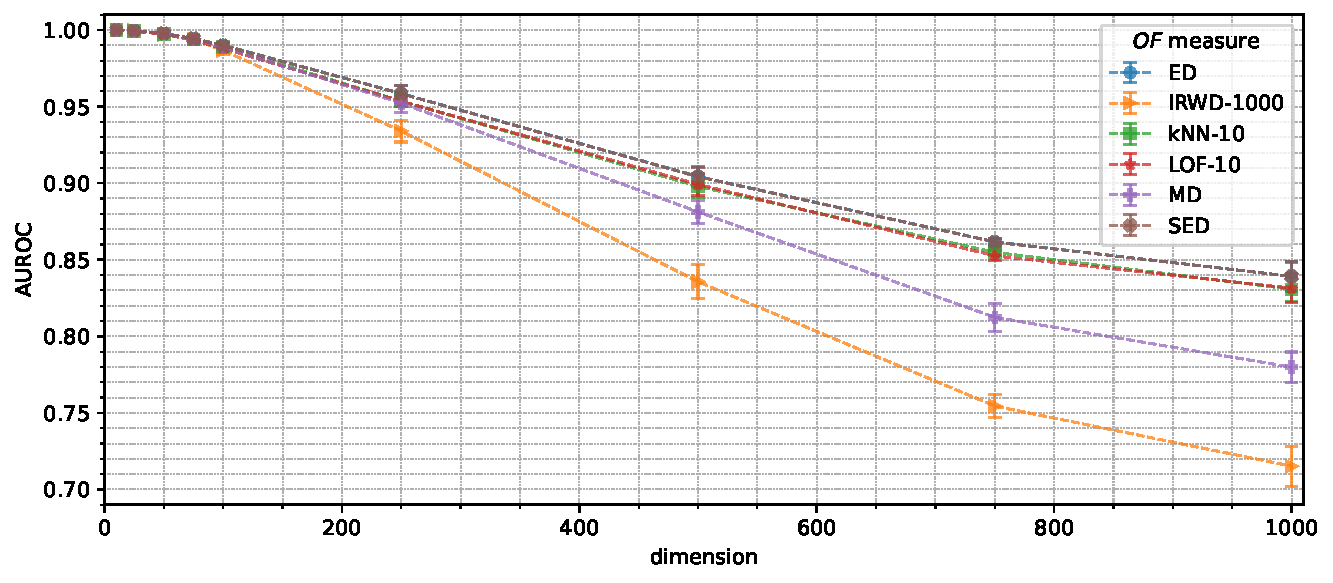
\includegraphics[width=\textwidth]{images/distributions/trends-d/trend-distributions-auroc(dimension)-samples_2500-distance_8-distribution_gaussian-model_ED,IRWD-1000,kNN-10,LOF-10,MD,SED-aggregated.pdf}
        \label{fig:dimension-auroc}
    \end{subfigure}
    \begin{subfigure}[b]{0.9\textwidth}
        % StreamLit settings: width=9, height=4
        % X: [0.00, 1010.00]
        % Y: [0.48, 1.00]
        \centering
        \caption{\small Classification with respect to the training data}
        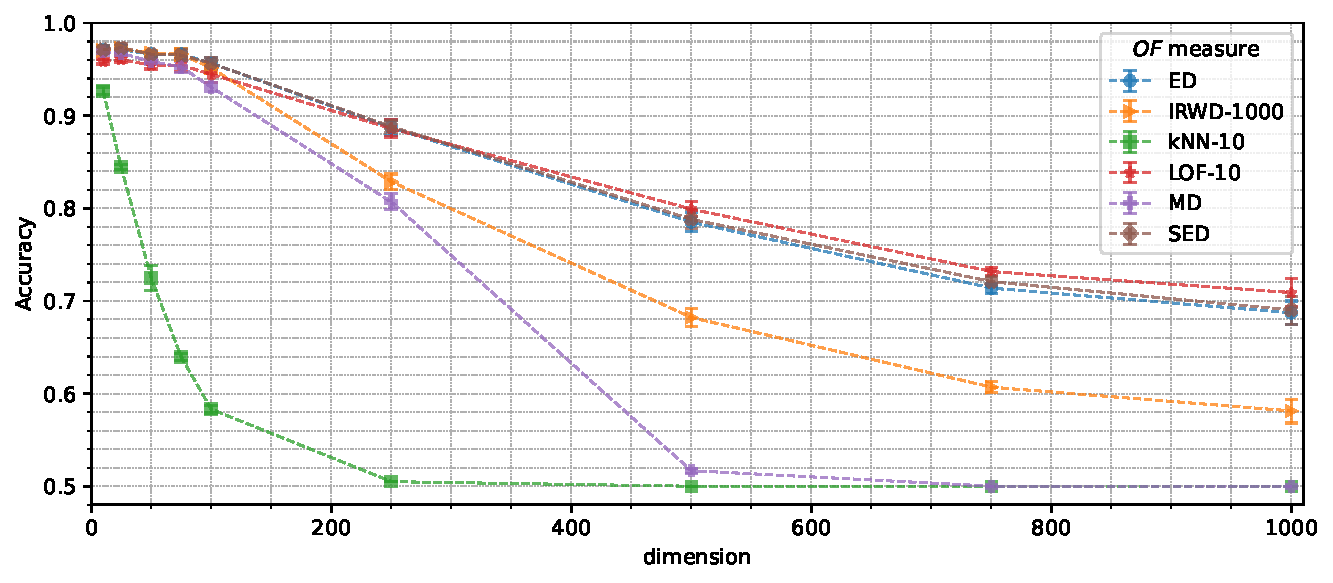
\includegraphics[width=\textwidth]{images/distributions/trends-d/trend-distributions-accuracy_95(dimension)-samples_2500-distance_8-distribution_gaussian-model_ED,IRWD-1000,kNN-10,LOF-10,MD,SED-aggregated.pdf}
        \label{fig:dimension-accuracy}
    \end{subfigure}
    \begin{subfigure}[b]{0.495\textwidth}
        % StreamLit settings: width=5, height=3
        % X: [0.00, 1010.00]
        % Y: [-0.02, 1.05]
        \centering
        \caption{\small Correctly recognized in-distribution}
        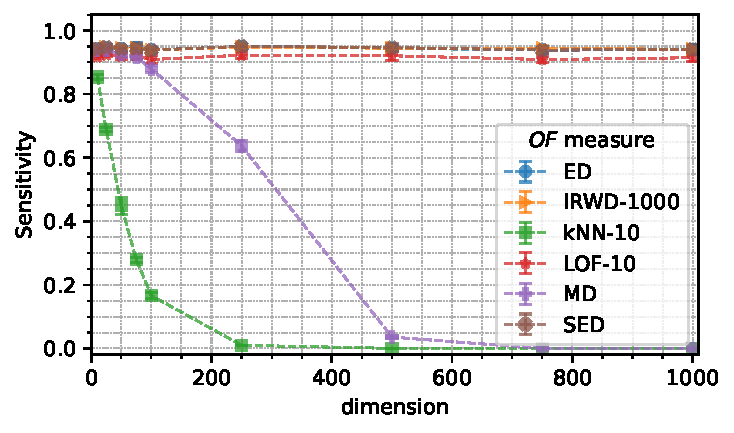
\includegraphics[width=\textwidth]{images/distributions/trends-d/trend-distributions-sens_95(dimension)-samples_2500-distance_8-distribution_gaussian-model_ED,IRWD-1000,kNN-10,LOF-10,MD,SED-aggregated.pdf}
        \label{fig:dimension-sensitivity}
    \end{subfigure}
    \hfill
    \begin{subfigure}[b]{0.495\textwidth}
        % StreamLit settings: width=5, height=3
        % X: [0.00, 1010.00]
        % Y: [-0.02, 1.05]
        \centering
        \caption{\small Correctly recognized out-of-distribution}
        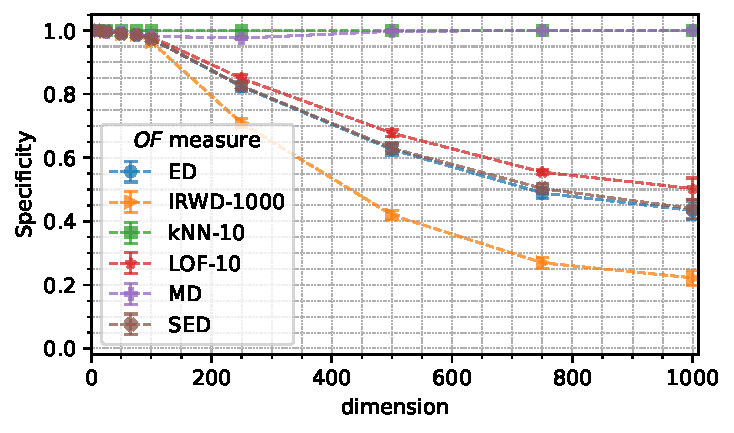
\includegraphics[width=\textwidth]{images/distributions/trends-d/trend-distributions-spec_95(dimension)-samples_2500-distance_8-distribution_gaussian-model_ED,IRWD-1000,kNN-10,LOF-10,MD,SED-aggregated.pdf}
        \label{fig:dimension-specificity}
    \end{subfigure}
    \caption{The performance of outlierness measures $OF$ as affected by the dimension of  the feature space $d$. The fixed parameters in the experiment are: number~of~training samples $n = 2500$, distance to outliers $h = 8$ and distribution $G = Gaussian$. The~results are aggregated for multiple generator seeds $\xi$ and~displayed as averages with~error~bars (standard deviation).}
    \label{fig:dimension}
    \vspace{-1.0em}
\end{figure}

\begin{figure}[t]
    % Query: samples >= 100 and samples <= 10000
    \centering
    \begin{subfigure}[b]{0.9\textwidth}
        % StreamLit settings: width=9, height=4
        % X: [95.00, 10500.00]
        % Y: [0.68, 0.88]
        \centering
        \caption{\small Separability between in-distribution and out-of-distribution data}
        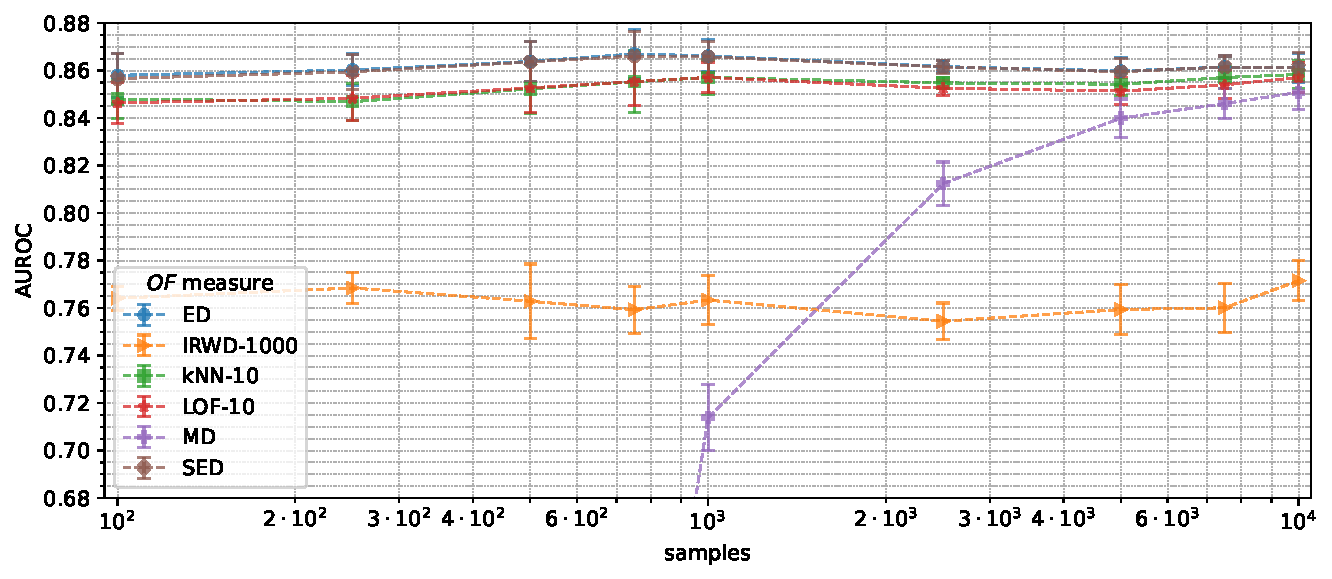
\includegraphics[width=\textwidth]{images/distributions/trends-n/trend-distributions-auroc(samples)-dimension_750-distance_8-distribution_gaussian-model_ED,IRWD-1000,kNN-10,LOF-10,MD,SED-aggregated.pdf}
        \label{fig:samples-auroc}
    \end{subfigure}
    \begin{subfigure}[b]{0.9\textwidth}
        % StreamLit settings: width=9, height=4
        % X: [95.00, 10500.00]
        % Y: [0,49, 0.80]
        \centering
        \caption{\small Classification with respect to the training data}
        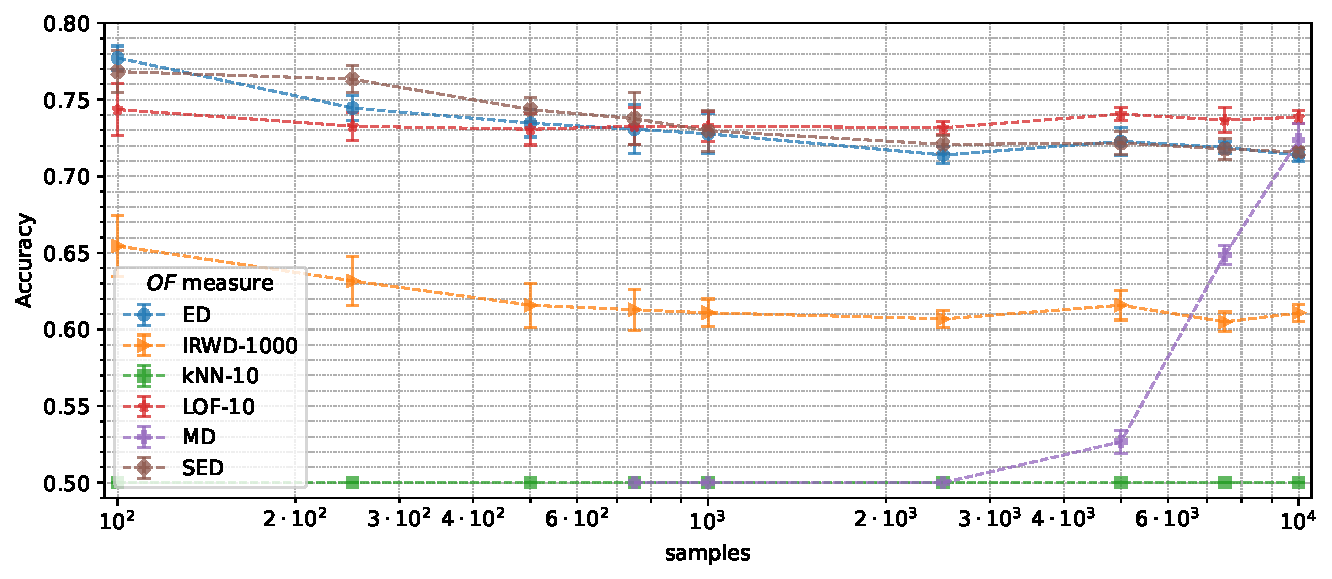
\includegraphics[width=\textwidth]{images/distributions/trends-n/trend-distributions-accuracy_95(samples)-dimension_750-distance_8-distribution_gaussian-model_ED,IRWD-1000,kNN-10,LOF-10,MD,SED-aggregated.pdf}
        \label{fig:samples-accuracy}
    \end{subfigure}
    \begin{subfigure}[b]{0.495\textwidth}
        % StreamLit settings: width=5, height=3
        % X: [95.00, 10500.00]
        % Y: [-0.02, 1.05]
        \centering
        \caption{\small Correctly recognized in-distribution}
        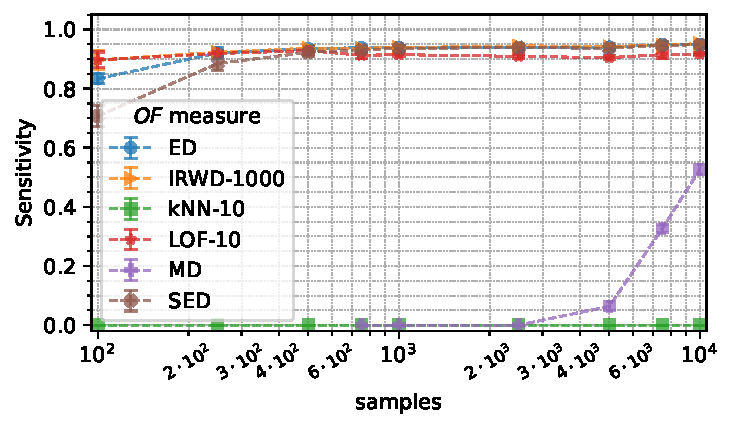
\includegraphics[width=\textwidth]{images/distributions/trends-n/trend-distributions-sens_95(samples)-dimension_750-distance_8-distribution_gaussian-model_ED,IRWD-1000,kNN-10,LOF-10,MD,SED-aggregated.pdf}
        \label{fig:samples-sensitivity}
    \end{subfigure}
    \hfill
    \begin{subfigure}[b]{0.495\textwidth}
        % StreamLit settings: width=5, height=3
        % X: [95.00, 10500.00]
        % Y: [-0.02, 1.05]
        \centering
        \caption{\small Correctly recognized out-of-distribution}
        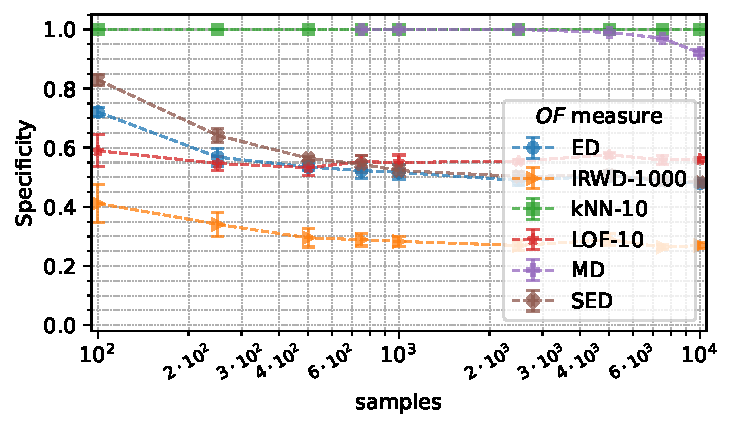
\includegraphics[width=\textwidth]{images/distributions/trends-n/trend-distributions-spec_95(samples)-dimension_750-distance_8-distribution_gaussian-model_ED,IRWD-1000,kNN-10,LOF-10,MD,SED-aggregated.pdf}
        \label{fig:samples-specificity}
    \end{subfigure}
    \caption{The performance of outlierness measures $OF$ as affected by the number of training samples $n$. The fixed parameters in the experiment are: dimension of the~feature space $d = 750$, distance to outliers $h = 8$ and distribution $G = Gaussian$. The~results are aggregated for multiple generator seeds $\xi$ and displayed as averages with~error~bars (standard deviation).}
    \label{fig:samples}
    \vspace{-1.0em}
\end{figure}

\begin{figure}[t]
    \centering
    \begin{subfigure}[b]{0.9\textwidth}
        % StreamLit settings: width=9, height=4
        % X: [0.96, 16.60]
        % Y: [0.46, 1.02]
        \centering
        \caption{\small Separability between in-distribution and out-of-distribution data}
        \includegraphics[width=\textwidth]{images/distributions/trends-h/trend-distributions-auroc(distance)-dimension_750-samples_2500-distribution_gaussian-model_ED,IRWD-1000,kNN-10,LOF-10,MD,SED-aggregated.pdf}
        \label{fig:distance-auroc}
    \end{subfigure}
    \begin{subfigure}[b]{0.9\textwidth}
        % StreamLit settings: width=9, height=4
        % X: [0.96, 16.60]
        % Y: [0,48, 1.00]
        \centering
        \caption{\small Classification with respect to the training data}
        \includegraphics[width=\textwidth]{images/distributions/trends-h/trend-distributions-accuracy_95(distance)-dimension_750-samples_2500-distribution_gaussian-model_ED,IRWD-1000,kNN-10,LOF-10,MD,SED-aggregated.pdf}
        \label{fig:distance-accuracy}
    \end{subfigure}
    \begin{subfigure}[b]{0.495\textwidth}
        % StreamLit settings: width=5, height=3
        % X: [0.96, 16.60]
        % Y: [-0.02, 1.05]
        \centering
        \caption{\small Correctly recognized in-distribution}
        \includegraphics[width=\textwidth]{images/distributions/trends-h/trend-distributions-sens_95(distance)-dimension_750-samples_2500-distribution_gaussian-model_ED,IRWD-1000,kNN-10,LOF-10,MD,SED-aggregated (1).pdf}
        \label{fig:distance-sensitivity}
    \end{subfigure}
    \hfill
    \begin{subfigure}[b]{0.495\textwidth}
        % StreamLit settings: width=5, height=3
        % X: [0.96, 16.60]
        % Y: [-0.02, 1.05]
        \centering
        \caption{\small Correctly recognized out-of-distribution}
        \includegraphics[width=\textwidth]{images/distributions/trends-h/trend-distributions-spec_95(distance)-dimension_750-samples_2500-distribution_gaussian-model_ED,IRWD-1000,kNN-10,LOF-10,MD,SED-aggregated.pdf}
        \label{fig:distance-specificity}
    \end{subfigure}
    \caption{The performance of outlierness measures $OF$ as affected by the distance to outliers $h$. The fixed parameters in the experiment are: dimension of the~feature space $d = 750$, number of training samples $n = 2500$ and distribution $G = Gaussian$. The~results are aggregated for multiple generator seeds $\xi$ and displayed as averages with~error~bars (standard deviation).}
    \label{fig:distance}
    \vspace{-1.0em}
\end{figure}

\cleardoublepage{}


\section{Effect of feature correlations}
\label{section:correlations-experiment}

The next experiment aims to analyze how the presence of correlations in data affects the~performance of outlier detection methods. The research is conducted considering various number of features correlated and various correlation strength, under fixed number of training samples and dimension of the feature vectors.


\subsection{Experiment organization}
\label{section:correlations-organization}

The experiment was organized similarly as the one described in the section \ref{section:distributions-organization}.

The difference lies in the definitions of datasets $T$, $K$ and $U$ – utilizing only one generator $G$ – the Multivariate Normal distribution (MVN). The number of training samples was fixed to $n = 2000$, as well as the dimension of feature vectors $d = 1000$. Instead, there are two new parameters introduced:
\vspace{-0.5\baselineskip}
\begin{itemize}
    \item the fraction of features that are correlated $f_{corr}$,
    \item the strength of the features correlation $g_{corr}$ (i.e., covariance value).
\end{itemize}

Both mentioned values affect the content of the covariance matrix $\Sigma$ that is supplied to the MVN generator, e.g., for $d = 8$, $f_{corr} = 0.5$ and $g_{corr} = 0.25$ it would become
\begin{equation}
    \Sigma_{ID}
    =
    \begin{bmatrix}
        \mathbf{1.00} & \mathbf{0.25} & \mathbf{0.25} & \mathbf{0.25} & 0.00 & 0.00 & 0.00 & 0.00 \\
        \mathbf{0.25} & \mathbf{1.00} & \mathbf{0.25} & \mathbf{0.25} & 0.00 & 0.00 & 0.00 & 0.00 \\
        \mathbf{0.25} & \mathbf{0.25} & \mathbf{1.00} & \mathbf{0.25} & 0.00 & 0.00 & 0.00 & 0.00 \\
        \mathbf{0.25} & \mathbf{0.25} & \mathbf{0.25} & \mathbf{1.00} & 0.00 & 0.00 & 0.00 & 0.00 \\
        0.00 & 0.00 & 0.00 & 0.00 & \mathbf{1.00} & 0.00 & 0.00 & 0.00 \\
        0.00 & 0.00 & 0.00 & 0.00 & 0.00 & \mathbf{1.00} & 0.00 & 0.00 \\
        0.00 & 0.00 & 0.00 & 0.00 & 0.00 & 0.00 & \mathbf{1.00} & 0.00 \\
        0.00 & 0.00 & 0.00 & 0.00 & 0.00 & 0.00 & 0.00 & \mathbf{1.00}
    \end{bmatrix}
    .
    \label{eq:corr-example}
\end{equation}

By default the features are not correlated and the variance of all features equals $1.0$.

Only the in-distribution (ID) data (sets $T$ and $K$) are affected by the new parameters. The out-of-distribution (OOD) examples (set $U$) utilizes the identity matrix during generation (i.e., $\Sigma_{OOD} = \mathbb{I}$, features uncorrelated, variance equal to $1.0$).

Summarizing, the input parameters that vary in the experiment are: the fraction of~features that are correlated $f_{corr}$, the strength of the correlation $g_{corr}$, the~distance to~the outliers $h$ and outlierness measure $OF$. The experiment was repeated several times with various values of the generator seed $\xi$.


\subsection{Experiment results}
\label{section:correlations-results}

Second experiment analyzes how the performance of outlierness measures is influenced by the correlations of features in dataset. Surprisingly, there are similarities noticeable when comparing the effect of changed correlation strength for a fixed number of correlated features (figure \ref{fig:covariance}) and the effect of changed fraction of correlated features for a fixed variance (figure \ref{fig:n_correlated}). The experiment involves $n = 2000$ training samples of dimension $d = 1000$ and distance to outliers $h = 8$.

In particular, the ED and SED behave nearly identically in both cases. The correlation of features in data results in more concentrated distribution along a selected direction in the feature space, having an effect similar to the reduction of dimensionality. However, in case of measures that do not consider the correlations, like ED or SED, the result is visible as more extended distribution in space. This effect can be seen in figures \ref{fig:hists-correlations-sed} and \ref{fig:hists-correlations-extreme-sed}. The outcome is worse separability (AUROC value) and classification accuracy for more correlated features, which is caused by the scores for out-of-distribution data appearing within the distribution obtained for training data (especially visible in figure \ref{fig:hists-correlations-extreme-sed}).

The kNN, LOF and MD measures are capable of benefiting from the correlated features, however the nature behind this effect is different. The result in all cases is that the separability of the data is better (greater AUROC values); in general LOF performs slightly better than kNN in this experiment and MD is obtaining the third best separability in most cases for correlated data, i.e., for $f_{corr} > 0.1$ and/or $g_{corr} > 0.1$ (for uncorrelated data, ED and SED performs better than MD here). The effect on AUROC is similar regardless of whether the faction of correlated featured is increased or correlation strength (covariance value) is greater, but for MD the effect is slightly stronger for greater covariance value – i.e., for $g_{corr} \geq 0.4$ it outperforms kNN in the task of separability (and for $g_{corr} \geq 0.5$ it even outperforms LOF). Yet, both kNN and MD are suffering in the task of classification with respect to the training data – due to the same phenomenon already discussed in section \ref{section:distributions-experiment}, i.e., zero sensitivity, all testing in-distribution data are spuriously considered as outliers.

In conducted experiment, only the LOF maintains the good accuracy in the classification task, benefiting from the correlated features. Comparing the figures \ref{fig:hists-correlations-lof} and \ref{fig:hists-correlations-extreme-lof}, it is because out-of-distribution data are seen as more distant in case of stronger correlation in the in-distribution dataset.

Interesting observation can be made when comparing figures \ref{fig:hists-correlations-knn} and \ref{fig:hists-correlations-extreme-knn} (kNN) with figures \ref{fig:hists-correlations-md} and \ref{fig:hists-correlations-extreme-md} (MD). In both cases the better separation between in-distribution test data and out-of-distribution samples is visible for more correlated features. However, in case of kNN, the effect of data concentration is visible – obtained score values for training data and known examples (clusters $T$ and $K$) are lower, corresponding with smaller spatial distances. Contrary, in case of MD, scores for both in-distribution data do not change significantly, yet still the outliers (cluster $U$) appears noticeably farther distanced.

\begin{figure}[t]
    \centering
    \begin{subfigure}[b]{0.9\textwidth}
        % StreamLit settings: width=9, height=4
        % X: [-0.01, 1.01]
        % Y: [0.69, 1.01]
        \centering
        \caption{\small Separability between in-distribution and out-of-distribution data}
        \includegraphics[width=\textwidth]{images/correlations/g_corr/trend-correlations-auroc(covariance)-n_correlated_0.20-distance_8-outliers_correlated_False-model_ED,IRWD-1000,kNN-10,LOF-10,MD,SED-aggregated.pdf}
        \label{fig:covariance-auroc}
    \end{subfigure}
    \begin{subfigure}[b]{0.9\textwidth}
        % StreamLit settings: width=9, height=4
        % X: [-0.01, 1.01]
        % Y: [0.44, 1.00]
        \centering
        \caption{\small Classification with respect to the training data}
        \includegraphics[width=\textwidth]{images/correlations/g_corr/trend-correlations-accuracy_95(covariance)-n_correlated_0.20-distance_8-outliers_correlated_False-model_ED,IRWD-1000,kNN-10,LOF-10,MD,SED-agg.pdf}
        \label{fig:covariance-accuracy}
    \end{subfigure}
    \begin{subfigure}[b]{0.495\textwidth}
        % StreamLit settings: width=5, height=3
        % X: [-0.01, 1.01]
        % Y: [-0.02, 1.05]
        \centering
        \caption{\small Correctly recognized in-distribution}
        \includegraphics[width=\textwidth]{images/correlations/g_corr/trend-correlations-sens_95(covariance)-n_correlated_0.20-distance_8-outliers_correlated_False-model_ED,IRWD-1000,kNN-10,LOF-10,MD,SED-aggregated.pdf}
        \label{fig:covariance-sensitivity}
    \end{subfigure}
    \hfill
    \begin{subfigure}[b]{0.495\textwidth}
        % StreamLit settings: width=5, height=3
        % X: [-0.01, 1.01]
        % Y: [-0.02, 1.05]
        \centering
        \caption{\small Correctly recognized out-of-distribution}
        \includegraphics[width=\textwidth]{images/correlations/g_corr/trend-correlations-spec_95(covariance)-n_correlated_0.20-distance_8-outliers_correlated_False-model_ED,IRWD-1000,kNN-10,LOF-10,MD,SED-aggregated.pdf}
        \label{fig:covariance-specificity}
    \end{subfigure}
    \caption{The performance of outlierness measures $OF$ as affected by the correlation strength (covariance value $g_{corr}$). The fixed parameters in the experiment are: dimension of the~feature space $d = 1000$, number of training samples $n = 2000$, distance to outliers $h = 8$ and fraction of features that are correlated $f_{corr} = 0.2$. The~results are aggregated for multiple generator seeds $\xi$ and displayed as averages with~error~bars (standard deviation).}
    \label{fig:covariance}
    \vspace{-2.3em}
\end{figure}

\begin{figure}[t]
    \centering
    \begin{subfigure}[b]{0.9\textwidth}
        % StreamLit settings: width=9, height=4
        % X: [-0.01, 1.01]
        % Y: [0.69, 1.01]
        \centering
        \caption{\small Separability between in-distribution and out-of-distribution data}
        \includegraphics[width=\textwidth]{images/correlations/f_corr/trend-correlations-auroc(n_correlated)-covariance_0.20-distance_8-outliers_correlated_False-model_ED,IRWD-1000,kNN-10,LOF-10,MD,SED-aggregated.pdf}
        \label{fig:n_correlated-auroc}
    \end{subfigure}
    \begin{subfigure}[b]{0.9\textwidth}
        % StreamLit settings: width=9, height=4
        % X: [-0.01, 1.01]
        % Y: [0.44, 1.00]
        \centering
        \caption{\small Classification with respect to the training data}
        \includegraphics[width=\textwidth]{images/correlations/f_corr/trend-correlations-accuracy_95(n_correlated)-covariance_0.20-distance_8-outliers_correlated_False-model_ED,IRWD-1000,kNN-10,LOF-10,MD,SED-agg.pdf}
        \label{fig:n_correlated-accuracy}
    \end{subfigure}
    \begin{subfigure}[b]{0.495\textwidth}
        % StreamLit settings: width=5, height=3
        % X: [-0.01, 1.01]
        % Y: [-0.02, 1.05]
        \centering
        \caption{\small Correctly recognized in-distribution}
        \includegraphics[width=\textwidth]{images/correlations/f_corr/trend-correlations-sens_95(n_correlated)-covariance_0.20-distance_8-outliers_correlated_False-model_ED,IRWD-1000,kNN-10,LOF-10,MD,SED-aggregated.pdf}
        \label{fig:n_correlated-sensitivity}
    \end{subfigure}
    \hfill
    \begin{subfigure}[b]{0.495\textwidth}
        % StreamLit settings: width=5, height=3
        % X: [-0.01, 1.01]
        % Y: [-0.02, 1.05]
        \centering
        \caption{\small Correctly recognized out-of-distribution}
        \includegraphics[width=\textwidth]{images/correlations/f_corr/trend-correlations-spec_95(n_correlated)-covariance_0.20-distance_8-outliers_correlated_False-model_ED,IRWD-1000,kNN-10,LOF-10,MD,SED-aggregated.pdf}
        \label{fig:n_correlated-specificity}
    \end{subfigure}
    \caption{The performance of outlierness measures $OF$ as affected by the fraction of features that are correlated $f_{corr}$. The fixed parameters in the experiment are: dimension of the~feature space $d = 1000$, number of training samples $n = 2000$, distance to outliers $h = 8$ and correlation strength (covariance value $g_{corr} = 0.2$). The~results are aggregated for multiple generator seeds $\xi$ and displayed as averages with~error~bars~(standard deviation).}
    \label{fig:n_correlated}
    \vspace{-2.3em}
\end{figure}

\begin{figure}[t]
    % StreamLit settings: width=9, height=2
    \centering
    \begin{subfigure}[b]{\textwidth}
        \centering
        \caption{\small k-Nearest Neighbors ($k=10$), covariance: $g_{corr} = 0.2$, fraction: $f_{corr} = 0.2$}
        \includegraphics[width=\textwidth]{images/correlations/hists/hist-correlations-n_correlated_0.20-covariance_0.20-distance_8-outliers_correlated_False-model_kNN-10-seed_0.pdf}
        \label{fig:hists-correlations-knn}
    \end{subfigure}
    \begin{subfigure}[b]{\textwidth}
        \centering
        \caption{\small Local Outlier Factor ($k=10$), covariance: $g_{corr} = 0.2$, fraction: $f_{corr} = 0.2$}
        \includegraphics[width=\textwidth]{images/correlations/hists/hist-correlations-n_correlated_0.20-covariance_0.20-distance_8-outliers_correlated_False-model_LOF-10-seed_0.pdf}
        \label{fig:hists-correlations-lof}
    \end{subfigure}
    \begin{subfigure}[b]{\textwidth}
        \centering
        \caption{\small Mahalanobis distance, covariance: $g_{corr} = 0.2$, fraction: $f_{corr} = 0.2$}
        \includegraphics[width=\textwidth]{images/correlations/hists/hist-correlations-n_correlated_0.20-covariance_0.20-distance_8-outliers_correlated_False-model_MD-seed_0.pdf}
        \label{fig:hists-correlations-md}
    \end{subfigure}
    \begin{subfigure}[b]{\textwidth}
        \centering
        \caption{\small Standardized Euclidean distance, covariance: $g_{corr} = 0.2$, fraction: $f_{corr} = 0.2$}
        \includegraphics[width=\textwidth]{images/correlations/hists/hist-correlations-n_correlated_0.20-covariance_0.20-distance_8-outliers_correlated_False-model_SED-seed_0.pdf}
        \label{fig:hists-correlations-sed}
    \end{subfigure}
    \caption{Distributions of outlierness scores for various measures $OF$ with a~small fraction of features slightly correlated. The correlation makes the generated clusters more concentrated in space, resulting in a better separability in case of kNN, LOF and~MD, except for SED that is not considering correlations (compare with figure \ref{fig:hists-correlations-extreme}). Other experiment parameters involved: dimension of feature space $d = 1000$, number of~training samples $n = 2000$, distance~to~outliers $h = 8$, generator seed $\xi = 0$.}
    \label{fig:hists-correlations}
\end{figure}

\begin{figure}[t]
    % StreamLit settings: width=9, height=2
    \centering
    \begin{subfigure}[b]{\textwidth}
        \centering
        \caption{\small k-Nearest Neighbors ($k=10$), covariance: $g_{corr} = 0.5$, fraction: $f_{corr} = 0.5$}
        \includegraphics[width=\textwidth]{images/correlations/hists-extreme/hist-correlations-n_correlated_0.50-covariance_0.50-distance_8-outliers_correlated_False-model_kNN-10-seed_0.pdf}
        \label{fig:hists-correlations-extreme-knn}
    \end{subfigure}
    \begin{subfigure}[b]{\textwidth}
        \centering
        \caption{\small Local Outlier Factor ($k=10$), covariance: $g_{corr} = 0.5$, fraction: $f_{corr} = 0.5$}
        \includegraphics[width=\textwidth]{images/correlations/hists-extreme/hist-correlations-n_correlated_0.50-covariance_0.50-distance_8-outliers_correlated_False-model_LOF-10-seed_0.pdf}
        \label{fig:hists-correlations-extreme-lof}
    \end{subfigure}
    \begin{subfigure}[b]{\textwidth}
        \centering
        \caption{\small Mahalanobis distance, covariance: $g_{corr} = 0.5$, fraction: $f_{corr} = 0.5$}
        \includegraphics[width=\textwidth]{images/correlations/hists-extreme/hist-correlations-n_correlated_0.50-covariance_0.50-distance_8-outliers_correlated_False-model_MD-seed_0.pdf}
        \label{fig:hists-correlations-extreme-md}
    \end{subfigure}
    \begin{subfigure}[b]{\textwidth}
        \centering
        \caption{\small Standardized Euclidean distance, covariance: $g_{corr} = 0.5$, fraction: $f_{corr} = 0.5$}
        \includegraphics[width=\textwidth]{images/correlations/hists-extreme/hist-correlations-n_correlated_0.50-covariance_0.50-distance_8-outliers_correlated_False-model_SED-seed_0.pdf}
        \label{fig:hists-correlations-extreme-sed}
    \end{subfigure}
    \caption{Distributions of outlierness scores for various measures $OF$ with a~half of~features highly correlated. The significant correlation results in much~better separability in case of kNN, LOF and~MD; in case of not considering correlations SED measure, a long right tail appears (compare with figure \ref{fig:hists-correlations}). Other experiment parameters involved: dimension of feature space $d = 1000$, number of~training samples $n = 2000$, distance~to~outliers $h = 8$, generator seed $\xi = 0$.}
    \label{fig:hists-correlations-extreme}
\end{figure}

\cleardoublepage{}

\section{Influence of non-uniform variance of features}
\label{section:variances-experiment}

The third experiment is focused on analyzing the impact of the non-standardized features on the performance of the out-of-distribution detection techniques. The research considers such factors as the number of features with modified variance (other than default value: $1.0$) and the modified variance's value itself. Similarly to previous experiment, the number of training samples and dimension of feature vectors are fixed.

\vspace{2.0em}  % NOTE: Just to expand the elements on page a little


\subsection{Experiment organization}
\label{section:variances-organization}

The experiment was organized similarly as the one described in the section \ref{section:distributions-organization}.

The difference lies in the definitions of datasets $T$, $K$ and $U$ – utilizing only one generator $G$ – the Multivariate Normal distribution (MVN). The number of training samples was fixed to $n = 2000$, as well as the dimension of feature vectors $d = 1000$. Instead, there are two new parameters introduced:
\vspace{-0.5\baselineskip}
\begin{itemize}
    \item the fraction of features that have modified (non-default) variance $f_{var}$,
    \item the value of the modified variance $g_{var}$.
\end{itemize}

Both mentioned values affect the content of the covariance matrix $\Sigma$ that is supplied to the MVN generator, e.g., for $d = 6$, $f_{var} = 0.5$ and $g_{var} = 0.25$ it would become
\begin{equation}
    \Sigma_{ID}
    =
    \begin{bmatrix}
        \mathbf{0.25} & 0.00 & 0.00 & 0.00 & 0.00 & 0.00 \\
        0.00 & \mathbf{0.25} & 0.00 & 0.00 & 0.00 & 0.00 \\
        0.00 & 0.00 & \mathbf{0.25} & 0.00 & 0.00 & 0.00 \\
        0.00 & 0.00 & 0.00 & \mathbf{1.00} & 0.00 & 0.00 \\
        0.00 & 0.00 & 0.00 & 0.00 & \mathbf{1.00} & 0.00 \\
        0.00 & 0.00 & 0.00 & 0.00 & 0.00 & \mathbf{1.00}
    \end{bmatrix}
    .
    \label{eq:var-example}
\end{equation}

The features are not correlated here and the default variance of features equals $1.0$.

Only the in-distribution (ID) data (sets $T$ and $K$) are affected by the new parameters. The out-of-distribution (OOD) examples (set $U$) utilizes the identity matrix during generation (i.e., $\Sigma_{OOD} = \mathbb{I}$, features uncorrelated, variance equal to $1.0$).

Summarizing, the input parameters that vary in the experiment are: the fraction of features with non-default variance $f_{var}$, the value of the non-default variance $g_{var}$, the~distance to the outliers $h$ and outlierness measure $OF$. The experiment was repeated several times with various values of the generator seed $\xi$.


\subsection{Experiment results}
\label{section:variances-results}

Third experiment verifies how the outlierness measures perform when affected by the non-uniform variances of features in the dataset, i.e., part of the features in the in-distribution samples utilize a different variance.

Figure \ref{fig:variance} illustrates how the variance value $g_{var}$ influences the performance of outlierness measures. The custom variance value $g_{var}$ is set on a fixed 20\% of features ($f_{var} = 0.2$), while the remaining 80\% features keep the default unitary variance ($1.0$). The experiment involves $n = 2000$ training samples of dimension $d = 1000$ and distance to outliers $h = 16$.

Cases where variance $g_{var} < 1.0$ correspond to concentrated distributions and therefore better spatial separation of data – perfect AUROC score (value $1.0$) is obtained even for IRWD measure (left part of figure \ref{fig:variance-auroc}), leading also to a higher classification accuracy (left part of figure \ref{fig:variance-accuracy}).

The results indicate significant decrease of separability where the custom variance $g_{var} > 1.0$ is applied (right part of figure \ref{fig:variance-auroc}) – especially in case of measures that assume the same significance and values range of each feature: ED, IRWD, kNN and LOF. This situation corresponds to the values of selected 20\% features from in-distribution data overlapping with values for the corresponding features from the out-of-distribution data. Relying on those features leads to losing the ability of proper outliers recognition (specificity) due to too wide spatial distribution of training data – the obtained distance scores for known in-distribution data and out-of-distribution samples start to overlap.

The MD and SED measures take into account the features variances and compensate their contribution to the spatial distance calculation, effectively distinguishing the in-distribution and out-of-distribution data based on the remaining 80\% of features that do not overlap. In the conducted study, SED performs slightly better than MD in the separation task (figure \ref{fig:variance-auroc}) and much better in the classification with respect to the training dataset (\ref{fig:variance-accuracy}). The latter is due to the MD's lack of sensitivity, discussed already in the previous sections of this dissertation (mismatch between scores obtained for training $T$ and testing $K$ in-distribution samples).

It shall be noticed, that due to how the AUROC score calculation is performed\footnote{Implementation detail: the \texttt{roc\_curve()} from scikit-learn library \cite{scikit-learn} assumes higher scores to be associated with a positive label, i.e., treating the scores like the class probability value returned by the classifier; if the scores have different interpretation, like in the conducted study (distance -~lower scores indicate positive class), the function parameters have to be adjusted, e.g., by inverting the labels; \url{https://scikit-learn.org/stable/modules/generated/sklearn.metrics.roc_curve.html}}, for variance value $g_{var} > 2.25$ (figure \ref{fig:variance-auroc}) the unusual value of $\text{AUROC} < 0.5$ can be observed in case of ED, IRWD, kNN and LOF. This corresponds to the distributions histograms visible in the figures \ref{fig:hists-variances-ed}, \ref{fig:hists-variances-knn} and \ref{fig:hists-variances-extreme} – the outlierness scores of in-distribution data are greater (located to the right) than the scores obtained for out-of-distribution data. The interpretation of~that case is: the out-of-distribution data are located closer to the training cluster $T$ center (e.g.~estimated mean) than the actual in-distribution samples. In some of such cases, the fine separability between the in-distribution data and the outliers can be made, such as in figures \ref{fig:hists-variances-extreme-ed} or \ref{fig:hists-variances-extreme-md}. Notably, in cases visible in figures \ref{fig:hists-variances-extreme-ed} and \ref{fig:hists-variances-extreme-sed}, both ED and SED preserve outlierness scores for in-distribution data in the same range, so the very good classification accuracy could be reached if the classification criteria (section \ref{section:verification}, formula \ref{eq:open-set-classification}) would have been revised accordingly.

In some of the observed conditions (figures \ref{fig:hists-variances-knn} and \ref{fig:hists-variances-extreme-md}) it is impossible to reliably calibrate kNN and MD for classification, because the scores obtained for out-of-distribution data are located between scores observed for training and testing in-distribution data.

Figure \ref{fig:n_varied} shows the performance of outlierness measures when a fraction of features $f_{var}$ contains a custom, fixed variance. The fixed variance value is $g_{var} = 1.5$; the remaining fraction of features maintains the default unitary variance ($1.0$). Like in previous example, the results are shown for case involving $n = 2000$ training samples of dimension $d = 1000$ and distance to outliers $h = 16$. The results in this case are analogous the previously discussed case, however now the parameter effect bears stronger impact on all the analyzed measures. Still, both MD and SED perform better than other measures in terms of data separation potential (figure \ref{fig:n_varied-auroc}), as long as the fraction of features with custom variance does not bring the outliers too close to the training data. For $f_{var} = 0.6$ the in-distribution data are non-distinguishable from the outliers for MD and SED; for ED, kNN and LOF the same effect was observed for~$f_{var} = 0.5$.

Overall, the experiment suggests that the analysis of variances and the standardization of data may be necessary to maintain optimal performance of methods such as IRWD, kNN and LOF, while measures like MD or SED work out of the box in the considered scenarios.

\begin{figure}[t]
    \centering
    \begin{subfigure}[b]{0.9\textwidth}
        % StreamLit settings: width=9, height=4
        % X: [0.2, 4.05]
        % Y: [-0.02, 1.02]
        \centering
        \caption{\small Separability between in-distribution and out-of-distribution data}
        \includegraphics[width=\textwidth]{images/variances/g_var/trend-variances-auroc(variance)-n_varied_0.20-distance_16-outliers_varied_False-model_ED,IRWD-1000,kNN-10,LOF-10,MD,SED-aggregated.pdf}
        \label{fig:variance-auroc}
    \end{subfigure}
    \begin{subfigure}[b]{0.9\textwidth}
        % StreamLit settings: width=9, height=4
        % X: [0.2, 4.05]
        % Y: [0.44, 1.00]
        \centering
        \caption{\small Classification with respect to the training data}
        \includegraphics[width=\textwidth]{images/variances/g_var/trend-variances-accuracy_95(variance)-n_varied_0.20-distance_16-outliers_varied_False-model_ED,IRWD-1000,kNN-10,LOF-10,MD,SED-aggregated.pdf}
        \label{fig:variance-accuracy}
    \end{subfigure}
    \begin{subfigure}[b]{0.495\textwidth}
        % StreamLit settings: width=5, height=3
        % X: [0.2, 4.05]
        % Y: [-0.02, 1.05]
        \centering
        \caption{\small Correctly recognized in-distribution}
        \includegraphics[width=\textwidth]{images/variances/g_var/trend-variances-sens_95(variance)-n_varied_0.20-distance_16-outliers_varied_False-model_ED,IRWD-1000,kNN-10,LOF-10,MD,SED-aggregated.pdf}
        \label{fig:variance-sensitivity}
    \end{subfigure}
    \hfill
    \begin{subfigure}[b]{0.495\textwidth}
        % StreamLit settings: width=5, height=3
        % X: [0.2, 4.05]
        % Y: [-0.02, 1.05]
        \centering
        \caption{\small Correctly recognized out-of-distribution}
        \includegraphics[width=\textwidth]{images/variances/g_var/trend-variances-spec_95(variance)-n_varied_0.20-distance_16-outliers_varied_False-model_ED,IRWD-1000,kNN-10,LOF-10,MD,SED-aggregated.pdf}
        \label{fig:variance-specificity}
    \end{subfigure}
    \caption{The performance of outlierness measures $OF$ as affected by variance of~features value $g_{var}$. The fixed parameters in the experiment are: dimension of~the~feature space $d = 1000$, number of training samples $n = 2000$, distance to~outliers $h = 16$ and fraction of features that have modified variance $f_{var} = 0.2$. The~results~are aggregated for multiple generator seeds $\xi$ and displayed as averages with~error~bars~(standard deviation).}
    \label{fig:variance}
    \vspace{-2.3em}
\end{figure}

\begin{figure}[t]
    \centering
    \begin{subfigure}[b]{0.9\textwidth}
        % StreamLit settings: width=9, height=4
        % X: [-0.01, 1.01]
        % Y: [-0.02, 1.02]
        \centering
        \caption{\small Separability between in-distribution and out-of-distribution data}
        \includegraphics[width=\textwidth]{images/variances/f_var/trend-variances-auroc(n_varied)-variance_1.50-distance_16-outliers_varied_False-model_ED,IRWD-1000,kNN-10,LOF-10,MD,SED-aggregated.pdf}
        \label{fig:n_varied-auroc}
    \end{subfigure}
    \begin{subfigure}[b]{0.9\textwidth}
        % StreamLit settings: width=9, height=4
        % X: [-0.01, 1.01]
        % Y: [0.44, 1.05]
        \centering
        \caption{\small Classification with respect to the training data}
        \includegraphics[width=\textwidth]{images/variances/f_var/trend-variances-accuracy_95(n_varied)-variance_1.50-distance_16-outliers_varied_False-model_ED,IRWD-1000,kNN-10,LOF-10,MD,SED-aggregated.pdf}
        \label{fig:n_varied-accuracy}
    \end{subfigure}
    \begin{subfigure}[b]{0.495\textwidth}
        % StreamLit settings: width=5, height=3
        % X: [-0.01, 1.01]
        % Y: [-0.02, 1.00]
        \centering
        \caption{\small Correctly recognized in-distribution}
        \includegraphics[width=\textwidth]{images/variances/f_var/trend-variances-sens_95(n_varied)-variance_1.50-distance_16-outliers_varied_False-model_ED,IRWD-1000,kNN-10,LOF-10,MD,SED-aggregated.pdf}
        \label{fig:n_varied-sensitivity}
    \end{subfigure}
    \hfill
    \begin{subfigure}[b]{0.495\textwidth}
        % StreamLit settings: width=5, height=3
        % X: [-0.01, 1.01]
        % Y: [-0.02, 1.05]
        \centering
        \caption{\small Correctly recognized out-of-distribution}
        \includegraphics[width=\textwidth]{images/variances/f_var/trend-variances-spec_95(n_varied)-variance_1.50-distance_16-outliers_varied_False-model_ED,IRWD-1000,kNN-10,LOF-10,MD,SED-aggregated.pdf}
        \label{fig:n_varied-specificity}
    \end{subfigure}
    \caption{The performance of outlierness measures $OF$ as affected by the fraction of features that have modified variance $f_{var}$. The fixed parameters in the experiment are: dimension of the feature space $d = 1000$, number of training samples $n = 2000$, distance to outliers $h = 16$ and variance of~features value $g_{var} = 1.5$. The~results are aggregated for multiple generator seeds $\xi$ and displayed as averages with~error~bars~(standard deviation).}
    \label{fig:n_varied}
    \vspace{-2.3em}
\end{figure}

\begin{figure}[t]
    % StreamLit settings: width=9, height=2
    \centering
    \begin{subfigure}[b]{\textwidth}
        \centering
        \caption{\small Euclidean distance, variance: $g_{var} = 3.0$, fraction: $f_{var} = 0.2$}
        \includegraphics[width=\textwidth]{images/variances/hists/hist-variances-n_varied_0.20-variance_3.00-distance_16-outliers_varied_False-model_ED-seed_0.pdf}
        \label{fig:hists-variances-ed}
    \end{subfigure}
    \begin{subfigure}[b]{\textwidth}
        \centering
        \caption{\small k-Nearest Neighbors ($k=10$), variance: $g_{var} = 3.0$, fraction: $f_{var} = 0.2$}
        \includegraphics[width=\textwidth]{images/variances/hists/hist-variances-n_varied_0.20-variance_3.00-distance_16-outliers_varied_False-model_kNN-10-seed_0.pdf}
        \label{fig:hists-variances-knn}
    \end{subfigure}
    \begin{subfigure}[b]{\textwidth}
        \centering
        \caption{\small Mahalanobis distance, variance: $g_{var} = 3.0$, fraction: $f_{var} = 0.2$}
        \includegraphics[width=\textwidth]{images/variances/hists/hist-variances-n_varied_0.20-variance_3.00-distance_16-outliers_varied_False-model_MD-seed_0.pdf}
        \label{fig:hists-variances-md}
    \end{subfigure}
    \begin{subfigure}[b]{\textwidth}
        \centering
        \caption{\small Standardized Euclidean distance, variance: $g_{var} = 3.0$, fraction: $f_{var} = 0.2$}
        \includegraphics[width=\textwidth]{images/variances/hists/hist-variances-n_varied_0.20-variance_3.00-distance_16-outliers_varied_False-model_SED-seed_0.pdf}
        \label{fig:hists-variances-sed}
    \end{subfigure}
    \caption{Histograms of outlierness scores for various measures $OF$ considering data distribution with a~small fraction of features having bigger variance. Due to bigger variance the outliers starts to overlap with in-distribution data in space, yet measures that consider the variance (MD, SED) maintain the ability to separate the clusters, while for kNN the outliers appear closer to training data than the known in-distribution examples. Other experiment parameters involved: dimension of feature space $d = 1000$, number of~training samples $n = 2000$, distance~to~outliers $h = 16$, generator seed $\xi = 0$.}
    \label{fig:hists-variances}
\end{figure}

\begin{figure}[t]
    % StreamLit settings: width=9, height=2
    \centering
    \begin{subfigure}[b]{\textwidth}
        \centering
        \caption{\small Euclidean distance, variance: $g_{var} = 4.0$, fraction: $f_{var} = 0.5$}
        \includegraphics[width=\textwidth]{images/variances/hists-extreme/hist-variances-n_varied_0.50-variance_4.00-distance_16-outliers_varied_False-model_ED-seed_0.pdf}
        \label{fig:hists-variances-extreme-ed}
    \end{subfigure}
    \begin{subfigure}[b]{\textwidth}
        \centering
        \caption{\small k-Nearest Neighbors ($k=10$), variance: $g_{var} = 4.0$, fraction: $f_{var} = 0.5$}
        \includegraphics[width=\textwidth]{images/variances/hists-extreme/hist-variances-n_varied_0.50-variance_4.00-distance_16-outliers_varied_False-model_kNN-10-seed_0.pdf}
        \label{fig:hists-variances-extreme-knn}
    \end{subfigure}
    \begin{subfigure}[b]{\textwidth}
        \centering
        \caption{\small Mahalanobis distance, variance: $g_{var} = 4.0$, fraction: $f_{var} = 0.5$}
        \includegraphics[width=\textwidth]{images/variances/hists-extreme/hist-variances-n_varied_0.50-variance_4.00-distance_16-outliers_varied_False-model_MD-seed_0.pdf}
        \label{fig:hists-variances-extreme-md}
    \end{subfigure}
    \begin{subfigure}[b]{\textwidth}
        \centering
        \caption{\small Standardized Euclidean distance, variance: $g_{var} = 4.0$, fraction: $f_{var} = 0.5$}
        \includegraphics[width=\textwidth]{images/variances/hists-extreme/hist-variances-n_varied_0.50-variance_4.00-distance_16-outliers_varied_False-model_SED-seed_0.pdf}
        \label{fig:hists-variances-extreme-sed}
    \end{subfigure}
    \caption{Histograms of outlierness scores for various measures $OF$ considering data distribution with a~significant fraction of features having very big variance. In~such conditions it is impossible to reliably calibrate kNN and MD for classification, while both ED and SED preserve scores for in-distribution data in the same range (however, the formula \ref{eq:open-set-classification} would have to be revised for classification). Other experiment parameters involved: dimension of feature space $d = 1000$, number of~training samples $n = 2000$, distance~to~outliers $h = 16$, generator seed $\xi = 0$.}
    \label{fig:hists-variances-extreme}
\end{figure}

\cleardoublepage{}

\section{Overlapping and accurate representations}
\label{section:overlapping-experiment}

The goal of the next experiment is to identify the required conditions for maintaining the matching representations of in-distribution samples, i.e., overlapping histograms for training and testing data presented in previous sections (e.g., figures \ref{fig:hists-md-samples}, \ref{fig:hists-knn-samples} and \ref{fig:hists-dimensions}). The research is conducted, considering primarily the dimensions of feature vectors $d$ and the number of samples $n$.

\vspace{2.0em}  % NOTE: Just to expand the elements on page a little


\subsection{Experiment organization}
\label{section:overlapping-organization}

The experiment is organized as follows:
\vspace{-0.5\baselineskip}
\begin{itemize}
    \item First, 2 data clusters are generated.
          \begin{itemize}
              \item Both datasets ($K_1$, $K_2$) are produced from the same chosen generator~$G$ (\textit{Gaussian} [uncorrelated], \textit{MVN} [with part of features correlated], \textit{triangular} or \textit{uniform} distribution – that is located around the~center of~the coordinate system $[0, 0, \dots, 0]$ with spread of $\pm 1$), each dataset containing $n$ samples of~dimension~$d$.
          \end{itemize}
    \item Then the bounding boxes around the clusters $K_1$ and $K_2$ are constructed.
    \item Next the common part of the bounding boxes for $K_1$ and $K_2$ is identified.
    \item The volumes of discovered boxes are calculated: $V_{K_1}$, $V_{K_2}$, $V_{K_1 \cap K_2}$.
          \begin{itemize}
              \item The boxes are hyperrectangles in $\mathbb{R}^d$ space, with volumes defined as
                    \begin{equation}
                        V_K = \prod_{j=1}^d l_j
                        ~,
                        \label{eq:hyperrectangle-volume}
                    \end{equation}
                    where $l_j$ is the length of the box's edge that is parallel to the $j$-th axis,
                    \begin{equation}
                        l_j
                        =
                        \max\big\{
                            K[*,j]
                        \big\}
                        -
                        \min\big\{
                            K[*,j]
                        \big\}
                        .
                        \label{eq:hyperrectangle-edge-length}
                    \end{equation}
              \item For high dimensions, e.g., $d \geq 1000$, the calculated volumes can become so huge that the values hit the overflow in memory (i.e., $\pm\infty$ in the Floating-Point Arithmetic [IEEE-754] \cite{IEEE-754-2019}\cite{Goldberg-1991}). Hence, in computation, for efficiency the logarithmic representation was involved,
                    \begin{equation}
                        {Vl}_K = log_{10}(V_K) = \sum_{j=1}^d log_{10}(l_j)
                        ~,
                        \label{eq:hyperrectangle-volume-log}
                    \end{equation}
                    where the result represent the order of magnitude, e.g., ${Vl}_K = 3$ means the volume is equal to $1000$ and ${Vl}_K = 21$ corresponds to a volume of ${10}^{21}$ units.
          \end{itemize}
    \item Finally the Jaccard index of the bounding boxes is calculated – also known as the Intersection over Union metric, defined as the ratio between the overlapping area/volume and the union of two areas/volumes,
          \begin{equation}
              J(K_1, K_2)
              =
              IoU(K_1, K_2)
              =
              \frac{
                  V_{K_1 \cap K_2}
              }{
                  V_{K_1 \cup K_2}
              }
              =
              \frac{
                  V_{K_1 \cap K_2}
              }{
                  V_{K_1} + V_{K_2} - V_{K_1 \cap K_2}
              }
              .
              \label{eq:jaccard-index}
          \end{equation}
\end{itemize}

Summarizing, the input parameters varying in the experiment are: number of~samples $n$, dimension of the feature space $d$ and the generator distribution $G$. The experiment was repeated several times with various values of the generator seed $\xi$ (that affected the values within $K_1$ and $K_2$) to observe the variability of results.


\subsection{Experiment results}
\label{section:overlapping-results}

The fourth experiment explores the properties of the high-dimensional spaces, analyzing the requirements for obtaining the accurate representations of the data clusters represented with the bounding boxes and previously discussed distance measures (section \ref{section:measures}).

Figure \ref{fig:overlapping-1} displays the non-intuitive phenomenon of difficulty related to obtaining matching (overlapping) representations of two data clusters produced by the same distribution. The idea is to construct bounding boxes around the generated clusters, i.e., identifying minimum and maximum values of each feature (vector component) and identify the common part (intersection) of those two boxes. Then, the ratio between the volume of identified common part and the total volume covered by the two boxes is~calculated – so called Jaccard index (formula \ref{eq:jaccard-index}).

It turns out, that obtaining accurate representations that way requires a~significant number of samples $n$ and becomes especially difficult in higher dimension $d$. In addition, while it is possible to accomplish this for the distributions generators with finite output domain ($G = Triangular$, $G = Uniform$), it becomes gradually challenging for the $G = Gaussian$ distribution ($G = MVN$ in general) even in dimensions like $d \sim 10$. Surprisingly, involving the correlations of features in the generator does not seem to influence this task significantly (compare figures \ref{fig:iou-gaussian-detailed} and \ref{fig:iou-correlated-detailed}), although in practice it results in more concentrated clusters with smaller distances between points.

Figure \ref{fig:tpr-gaussian-md} presents a different attempt for obtaining a cluster representation, based on the training and testing data (clusters $T$ and $K$) from experiment described in section \ref{section:distributions-experiment}. In this approach, the clusters are represented using the Mahalanobis distance model, assuming hyperellipsoid-like structure of data, estimated using the covariance matrix and distances of the clusters points with respect to the ellipsoid center (mean values of features). Instead of Jaccard index, the sensitivity (True Positive Rate) is reported – counting the point from the testing cluster as from the same distribution, if it not farther than $99\%$ of the training data.

Utilizing this approach, achieving the accurate representation of the clusters is possible when providing sufficiently large number of samples $n$ for a given dimension $d$ of feature space. Surprisingly, the observed relation is very similar to the bounding boxes estimation obtained for $G = Uniform$ distribution (compare \ref{fig:iou-uniform} and \ref{fig:tpr-gaussian-md}). Note that reaching the accurate representation requires significantly more samples $n$ than the bare minimum required for estimating the covariance matrix in dimension $d$ –~minimum: $n \geq d$; optimum: $n \gtrsim 50 \cdot d$ (as for analyzed range in figure \ref{fig:tpr-gaussian-md}). This observation corresponds the phenomenon presented previously in figure \ref{fig:hists-md-samples} and justifies the utilization of the pooled covariance matrix when calculating Mahalanobis distance (section \ref{section:Mahalanobis}, formula \ref{eq:mdp}), as obtaining more samples can lead to more accurate representation of the training cluster and higher classifier sensitivity.

Figure \ref{fig:overlapping-3} presents comparison of other attempts of obtaining a~cluster representation using the distance measures described in~section \ref{section:measures}.
Figure \ref{fig:tpr-gaussian-knn} illustrates the previously discussed phenomenon of kNN measure mismatching between training and testing samples coming from the same distribution, depending on the chosen parameter $k$ value, as visible also in figure \ref{fig:hists-knn-samples}. In case of $k = 10$, any number of samples $n \geq 500$ does not improve the sensitivity (True Positive Rate). For greater $k$ values, the overall trend is preserved but appears shifted to the right in the figure, e.g., reaching $TPR \approx 0.9$ for $k = 20$ and $d = 100$. This observation deserves a~dedicated, separate further study.

Interestingly, the LOF measure appears nearly unaffected by dimensionality of the feature space in this task, reaching good score for all but extreme case ($n = 10$). The SED measure shows behavior similar to MD for the analyzed dimensions $d$ range, however the number of samples $n$ necessary to obtain accurate representation is much lower than for MD. This corresponds with the results observed in figures \ref{fig:hists-sed-dimensions}, \ref{fig:hists-sed-n50} and \ref{fig:hists-sed-n1000} in subsection \ref{section:distributions-results-properties}.

\begin{figure}[t]
    % StreamLit settings: width=9, height=4
    % X: [0.95, 10500.00]
    % Y: [-0.02, 1.02]
    \centering
    \vspace{-0.75em}
    \begin{subfigure}[b]{0.9\textwidth}
        \centering
        \caption{\small Distribution $G = Gaussian$}
        \includegraphics[width=\textwidth]{images/overlapping/trend-overlapping-IoU(dimension)-distribution_gaussian-samples_10,50,100,500,1000,5000,10000,50000-aggregated.pdf}
        \label{fig:iou-gaussian}
    \end{subfigure}

    \vspace{-0.75em}
    \begin{subfigure}[b]{0.9\textwidth}
        \centering
        \caption{\small Distribution $G = Triangular$}
        \includegraphics[width=\textwidth]{images/overlapping/trend-overlapping-IoU(dimension)-distribution_triangular-samples_10,50,100,500,1000,5000,10000,50000-aggregated.pdf}
        \label{fig:iou-triangular}
    \end{subfigure}

    \vspace{-0.75em}
    \begin{subfigure}[b]{0.9\textwidth}
        \centering
        \caption{\small Distribution $G = Uniform$}
        \includegraphics[width=\textwidth]{images/overlapping/trend-overlapping-IoU(dimension)-distribution_uniform-samples_10,50,100,500,1000,5000,10000,50000-aggregated.pdf}
        \label{fig:iou-uniform}
    \end{subfigure}

    \vspace{-0.5em}
    \caption{The relation between number of samples $n$ and dimension of feature space $d$ in the~task of recreating the same data cluster (represented as the bounding box). This task turns out significantly more difficult for $G = Gaussian$ distribution than for the distributions with finite output domain ($G = Triangular$, $G = Uniform$). The~results are aggregated for multiple generator seeds $\xi$ and displayed as averages with~error~bars~(standard deviation).}
    \label{fig:overlapping-1}
    \vspace{-3.2em}
\end{figure}

\begin{figure}[t]
    % StreamLit settings: width=9, height=4
    % X: [0.95, 10500.00]
    % Y: [-0.02, 1.02]
    \centering
    \vspace{-0.75em}
    \begin{subfigure}[b]{0.9\textwidth}
        \centering
        \caption{\small Distribution $G = Gaussian$ (detailed view)}
        \includegraphics[width=\textwidth]{images/overlapping/trend-overlapping-IoU(dimension)-distribution_gaussian-samples_10,50,100,500,1000,5000,10000,50000-aggregated-detailed.pdf}
        \label{fig:iou-gaussian-detailed}
    \end{subfigure}

    \vspace{-0.75em}
    \begin{subfigure}[b]{0.9\textwidth}
        \centering
        \caption{\small Distribution $G = MVN$ ($g_{corr} = 0.5$, $f_{corr} = 0.5$)}
        \includegraphics[width=\textwidth]{images/overlapping/trend-overlapping-IoU(dimension)-distribution_correlated-50-50-samples_10,50,100,500,1000,5000,10000,50000-aggregated-detailed.pdf}
        \label{fig:iou-correlated-detailed}
    \end{subfigure}

    \vspace{-0.75em}
    \begin{subfigure}[b]{0.9\textwidth}
        \centering
        \caption{\small Distribution $G = Gaussian$, utilizing Mahalanobis distance}
        \includegraphics[width=\textwidth]{images/overlapping/trend-distributions-sens_99(dimension)-distance_8-distribution_gaussian-model_MD-samples_10,50,100,500,1000,5000,10000,50000-aggregated.pdf}
        \label{fig:tpr-gaussian-md}
    \end{subfigure}

    \vspace{-0.5em}
    \caption{The correlation of features, despite resulting in more concentrated clusters (smaller distances), is does not affect the results significantly (comparing subfigures \ref{fig:iou-gaussian-detailed} and \ref{fig:iou-correlated-detailed}). However, representing cluster with Mahalanobis distance model (i.e., hyperellipsoid-like structure), the overlapping can be effectively achieved ever for higher dimensions $d$. The~results are aggregated for multiple generator seeds $\xi$ and displayed as averages with~error~bars~(standard deviation).}
    \label{fig:overlapping-2}
    \vspace{-3.2em}
\end{figure}

\begin{figure}[t]
    % StreamLit settings: width=9, height=4
    % X: [0.95, 10500.00]
    % Y: [-0.02, 1.02]
    \centering
    \vspace{-0.75em}
    \begin{subfigure}[b]{0.9\textwidth}
        \centering
        \caption{\small Distribution $G = Gaussian$, utilizing k-Nearest Neighbors ($k=10$)}
        \includegraphics[width=\textwidth]{images/overlapping/trend-distributions-sens_99(dimension)-distance_1-distribution_gaussian-model_kNN-10-samples_10,50,100,500,1000,5000,10000,50000-aggregated.pdf}
        \label{fig:tpr-gaussian-knn}
    \end{subfigure}

    \vspace{-0.75em}
    \begin{subfigure}[b]{0.9\textwidth}
        \centering
        \caption{\small Distribution $G = Gaussian$, utilizing Local Outlier Factor ($k=10$)}
        \includegraphics[width=\textwidth]{images/overlapping/trend-distributions-sens_99(dimension)-distance_1-distribution_gaussian-model_LOF-10-samples_10,50,100,500,1000,5000,10000,50000-aggregated.pdf}
        \label{fig:tpr-gaussian-lof}
    \end{subfigure}

    \vspace{-0.75em}
    \begin{subfigure}[b]{0.9\textwidth}
        \centering
        \caption{\small Distribution $G = Gaussian$, utilizing Standardized Euclidean distance}
        \includegraphics[width=\textwidth]{images/overlapping/trend-distributions-sens_99(dimension)-distance_1-distribution_gaussian-model_SED-samples_10,50,100,500,1000,5000,10000,50000-aggregated.pdf}
        \label{fig:tpr-gaussian-sed}
    \end{subfigure}

    \vspace{-0.5em}
    \caption{Clusters representations based on the distance measures described in~section \ref{section:measures} allow to obtain the effective overlapping ever for high features space dimensions $d$. For some methods the number of samples $n$ does not need to be high to~perform well; kNN's performance is related it selected parameter $k$ value. The~results are~aggregated for multiple generator seeds $\xi$ and displayed as averages with~error~bars~(standard deviation).}
    \label{fig:overlapping-3}
    \vspace{-3.2em}
\end{figure}

\cleardoublepage{}

\section{Parameter estimation errors}
\label{section:estimation-experiment}

The goal of the last numerical experiment is to explain the reason behind low sensitivity of MD, especially when compared with conceptually similar SED measure, e.g., visible when comparing the histograms in figures \ref{fig:hists-correlations-md} and \ref{fig:hists-correlations-sed}, also observing the rapid sensitivity decay for MD in higher dimensions $d$ in figure \ref{fig:dimension-sensitivity}. Both mentioned measures rely on estimating the vector of means $\mu$ and either the full covariance matrix $\Sigma$ or only its diagonal elements (variances). The analysis of errors impact is conducted as a function of the~feature space dimension $d$ and the~number of samples $n$.

\vspace{2.0em}  % NOTE: Just to expand the elements on page a little


\subsection{Experiment organization}
\label{section:estimation-organization}

The experiment is organized as follows:
\vspace{-0.5\baselineskip}
\begin{itemize}
    \item First, a single data cluster $K$ is generated.
          \begin{itemize}
              \item The dataset is produced from the Multivariate Normal distribution (MVN), containing $n$ samples of~dimension~$d$, located around the~center of~the coordinate system $\mu = [0, 0, \dots, 0]$ with a spread of $\pm 1$).
              \item The distribution shape is influenced by two additional parameters:
                    \begin{itemize}
                        \item the fraction of features that are correlated $f_{corr}$,
                        \item the strength of the features correlation $g_{corr}$.
                    \end{itemize}
                    These parameters affect the content of the covariance matrix $\Sigma$ supplied to the MVN generator, e.g., for $d = 5$, $f_{corr} = 0.6$ and $g_{corr} = 0.25$ it results in
                    \begin{equation}
                        \Sigma
                        =
                        \begin{bmatrix}
                            \mathbf{1.00} & \mathbf{0.25} & \mathbf{0.25} & 0.00 & 0.00 \\
                            \mathbf{0.25} & \mathbf{1.00} & \mathbf{0.25} & 0.00 & 0.00 \\
                            \mathbf{0.25} & \mathbf{0.25} & \mathbf{1.00} & 0.00 & 0.00 \\
                            0.00 & 0.00 & 0.00 & \mathbf{1.00} & 0.00 \\
                            0.00 & 0.00 & 0.00 & 0.00 & \mathbf{1.00}
                        \end{bmatrix}
                        .
                        \label{eq:corr-example-2}
                    \end{equation}
          \end{itemize}
    \item The sample mean $\hat{\mu}$ and empirical covariance $\hat{\Sigma}$ are estimated on the dataset $K$.
    \item The Mean Squared Error (MSE) of the estimates are calculated as per formula,
          \begin{equation}
              MSE(A, \hat{A})
              =
              \frac{1}{w}
              \cdot
              \sum_{i=1}^{w}
              \left(
                  A_i - \hat{A}_i
              \right)^2
              ,
              \label{eq:MSE}
          \end{equation}
          where $A$ is the true/expected value of a~parameter and $\hat{A}$ is its estimated value, $w$~is~the~number of components if $A$ is a~vector or matrix, $i$ indexes the components. In~particular, the inaccuracies of the~following parameters were computed:
          \begin{itemize}
              \item means: $MSE(\mu, \hat{\mu})$;
                    $w = d$;
              \item covariance matrices: $MSE(\Sigma, \hat{\Sigma})$;
                    $w = d^2$;
              \item variances: $MSE(\Sigma_{i,j}, \hat{\Sigma}_{i,j})$
                    where
                    $\forall (i, j) \in \{1, 2, \dots, d\}: i = j$;
                    $w = d$;
              \item correlations: $MSE(\Sigma_{i,j}, \hat{\Sigma}_{i,j})$
                    where
                    $\forall (i, j) \in \{1, 2, \dots, d\}: i \neq j$;
                    $w = \frac{d}{d - 1}$.
          \end{itemize}
\end{itemize}

Summarizing, the input parameters that vary in the experiment are: the number of~samples $n$, dimension of the feature space $d$, the fraction of~features that are correlated $f_{corr}$ and the strength of the correlation $g_{corr}$. The experiment was repeated several times with various values of the generator seed $\xi$.


\subsection{Experiment results}
\label{section:estimation-results}

The fifth experiment is a numerical study of how accurate the empirical estimations of distribution properties are, considering number of samples in cluster $n$ and the dimension $d$ of vectors, focusing in the high-dimensional feature spaces in particular.

Figure \ref{fig:estimation} presents the results obtained for a Multi-variate Normal (MVN) distribution with small fraction of features $f_{corr} = 0.2$ slightly correlated $g_{corr} = 0.2$. The experiment is conducted for a range of correlation settings and the results do not differ significantly – unless a very strong correlation of features in data is involved (as shown in the figure \ref{fig:estimation-strong}.

Surprisingly, all three analyzed parameters: means, variances and covariances; are estimated with similar accuracy for a given experiment configuration ($n$, $d$, $f_{corr}$, $g_{corr}$). The estimation errors are primarily related to the number of available data samples $n$, with the behavior being inversely proportional – the more examples provided, the lesser error (more accurate representation of the original/expected values). The estimation accuracy appears not significantly affected by the dimensionality of the feature space.

Comparing the results side-by-side (figures \ref{fig:estimation-means}, \ref{fig:estimation-variances} and \ref{fig:estimation-covariances}) it can be noticed that the estimation errors for means and covariances appear nearly the same, especially for higher dimensionality ($d \geq 100$), while the estimation of variances appear slightly worse (higher error). However, all estimation errors for a given set of parameters ($n$, $d$, $f_{corr}$, $g_{corr}$) are of the same order of magnitude.

\clearpage  % NOTE: To avoid splitting the list between pages

\begin{itemize}
    \item $d = 1000$, $f_{corr} = 0.2$, $g_{corr} = 0.2$, $n = 1000$:
          \begin{itemize}
              \item $MSE( \text{means} ) \approx 1.0 \cdot 10^{-3}$,
              \item $MSE( \text{variances} ) \approx 0.9 \cdot 10^{-3}$,
              \item $MSE( \text{covariances} ) \approx 1.0 \cdot 10^{-3}$;
          \end{itemize}
    \item $d = 1000$, $f_{corr} = 0.2$, $g_{corr} = 0.2$, $n = 10000$:
          \begin{itemize}
              \item $MSE( \text{means} ) \approx 1.0 \cdot 10^{-4}$,
              \item $MSE( \text{variances} ) \approx 0.9 \cdot 10^{-4}$,
              \item $MSE( \text{covariances} ) \approx 1.0 \cdot 10^{-4}$.
          \end{itemize}
\end{itemize}

This observation is significant, because when considering how the computed values are involved in the distances calculation for the MD measure (section \ref{section:Mahalanobis}, formula \ref{eq:md}) or the SED measure (section \ref{section:SEuclidean}, formula \ref{eq:sed}), the various cumulative error can be estimated. Assuming the average estimation error of a single parameter, e.g., the variance on the $j$-th axis or the covariance between features $j_1$ and $j_2$ (element $\Sigma_{j_1,j_2}$), being $\delta$ in both cases (same order of magnitude), when computing the Standardized Euclidean distance, each of the $d$ estimated variances scales the corresponding distances (vector components) that are later summed up, leading to a total cumulative error
\begin{equation}
    Err( \text{SED} )
    \approx
    \underbrace{
        \vphantom{\frac{a}{b}}  % Spacing hack – moves the underbrace a little down
        \delta + \delta + \dots + \delta
    }_{d~\text{components}}
    = d \cdot \delta
    \quad
    \sim
    \order{ d },
    \label{eq:sed-error}
\end{equation}
while the Mahalanobis distance formula (matrix times vector) involves $d$ multiplications and additions for each of the $d$ vector components, leading to a total cumulative error
\begin{equation}
    Err( \text{MD} )
    \approx
    \underbrace{
        \vphantom{\frac{a}{b}}  % Spacing hack – moves the underbrace a little down
        d \cdot \delta + d \cdot \delta + \dots + d \cdot \delta
    }_{d~\text{components}}
    = d^2 \cdot \delta
    \quad
    \sim
    \order{ d^2 }.
    \label{eq:md-error}
\end{equation}

Hence, summarizing, as long as no significant correlation of feature is involved, the SED appears to~be preferable than MD, promising more accurate distance calculation in high-dimensional feature spaces.

The obtained results justifies why it is worth to increase the number of training samples $n$ for the estimation of covariance matrix $\Sigma$, and hence the utilization of pooled covariance matrix is motivated, i.e., single common covariance matrix assumed for all in-distribution classes (MDP measure, section \ref{section:Mahalanobis}). However, as it is shown in next chapter, the latter mentioned approach suffers also from the other kind of method error.

\begin{figure}[t]
    % StreamLit settings: width=9, height=4
    % X: [0.95, 10500.00]
    % Y: [0,000005, 1.20]
    \centering
    \vspace{-0.5em}
    \begin{subfigure}[b]{0.9\textwidth}
        \centering
        \caption{\small Error estimating means}
        \includegraphics[width=\textwidth]{images/estimation/trend-properties-mse_means(dimension)-n_correlated_0.20-covariance_0.20-samples_10,50,100,500,1000,5000,10000,50000-aggregated.pdf}
        \label{fig:estimation-means}
    \end{subfigure}

    \vspace{-0.5em}
    \begin{subfigure}[b]{0.9\textwidth}
        \centering
        \caption{\small Error estimating variances}
        \includegraphics[width=\textwidth]{images/estimation/trend-properties-mse_vars(dimension)-n_correlated_0.20-covariance_0.20-samples_10,50,100,500,1000,5000,10000,50000-aggregated.pdf}
        \label{fig:estimation-variances}
    \end{subfigure}

    \vspace{-0.5em}
    \begin{subfigure}[b]{0.9\textwidth}
        \centering
        \caption{\small Error estimating covariances}
        \includegraphics[width=\textwidth]{images/estimation/trend-properties-mse_covs(dimension)-n_correlated_0.20-covariance_0.20-samples_10,50,100,500,1000,5000,10000,50000-aggregated.pdf}
        \label{fig:estimation-covariances}
    \end{subfigure}

    \vspace{-0.5em}
    \caption{The estimation errors of selected cluster properties. The cluster contains $n$ samples of dimension $d$, generated from $G = MVN$ distribution with small fraction of features $f_{corr} = 0.2$ slightly correlated $g_{corr} = 0.2$. The more $n$ samples provided, the~more accurate estimation. The~results are aggregated for multiple generator seeds $\xi$ and displayed as averages with~error~bars~(standard deviation).}
    \label{fig:estimation}
    \vspace{-2.5em}
\end{figure}

\begin{figure}[t]
    % StreamLit settings: width=9, height=4
    % X: [0.95, 10500.00]
    % Y: [0,000005, 1.20]
    \centering
    \vspace{-0.5em}
    \begin{subfigure}[b]{0.9\textwidth}
        \centering
        \caption{\small Error estimating means}
        \includegraphics[width=\textwidth]{images/estimation/trend-properties-mse_means(dimension)-n_correlated_0.80-covariance_0.80-samples_10,50,100,500,1000,5000,10000,50000-aggregated.pdf}
        \label{fig:estimation-strong-means}
    \end{subfigure}

    \vspace{-0.5em}
    \begin{subfigure}[b]{0.9\textwidth}
        \centering
        \caption{\small Error estimating variances}
        \includegraphics[width=\textwidth]{images/estimation/trend-properties-mse_vars(dimension)-n_correlated_0.80-covariance_0.80-samples_10,50,100,500,1000,5000,10000,50000-aggregated.pdf}
        \label{fig:estimation-strong-variances}
    \end{subfigure}

    \vspace{-0.5em}
    \begin{subfigure}[b]{0.9\textwidth}
        \centering
        \caption{\small Error estimating covariances}
        \includegraphics[width=\textwidth]{images/estimation/trend-properties-mse_covs(dimension)-n_correlated_0.80-covariance_0.80-samples_10,50,100,500,1000,5000,10000,50000-aggregated.pdf}
        \label{fig:estimation-strong-covariances}
    \end{subfigure}

    \vspace{-0.5em}
    \caption{The estimation errors of selected cluster properties. The cluster contains $n$ samples of dimension $d$, generated from $G = MVN$ distribution with great fraction of features $f_{corr} = 0.8$ highly correlated $g_{corr} = 0.8$. Under strong correlation, results are less stable, yet remaining of the same order. The~results are aggregated for multiple generator seeds $\xi$ and displayed as averages with~error~bars~(standard deviation).}
    \label{fig:estimation-strong}
    \vspace{-2.5em}
\end{figure}

\cleardoublepage{}



\section{Reproducibility of results}
\label{section:reproductibility}

All experiments were conducted several times to ensure that the overall patterns and trends were captured, rather than observing a single specific exception – hence the error bars were drawn on plots in this chapter. Additionally, all initialization parameters for the involved pseudo-random number generators (PRNGs) were recorded, so any examined case can be recreated and inspected further in another study, utilizing the~tools described in~appendix \ref{chapter:source-code}.
